\chapter[Leçon 39: Ernierung, Hausdéieren, Gesondheet \& A1-Grondlagen]{Leçon 39: Ernierung, Kachen, Hausdéieren, Gesondheet \& A1-Grondlagen (Verben, Artikelen a Negatioun)}

Dës Lektioun behandelt zwee grouss Schwéierpunkter vum Lëtzebuergeschen mat hire grammateschen a lexikalesche Feinheeten. Am éischten Deel geet et ëm dräi grouss Konversatiouns- a Sproochentest-Sujete : \textbf{Ernierung, Fastfood a Kachen doheem} (Moiesiessen, Eeër-Variatiounen, syyresch Spezialitéite wéi Hummus a Falafel, an de wichtegen Ënnerscheed tëscht \textit{gär hunn} an dem däitsche Faux-ami \textit{*lieben}), \textbf{Hausdéieren a Gesondheet} (Vergaangenheetsforme mat \textit{fréier} a \textit{virdrun}, de Präteritum \textit{ech hat}, an d'Aussprooch vun \textit{d'Hoer} vs. \textit{d'Ouer}), souwéi \textbf{Krankheet, Dokter an Hausmëttelen} (\textit{dacks}, \textit{oft} a \textit{meeschtens}, Medikamenter \textit{huelen}, Téi mat Ingwer, Zitroun, Peffermënz an Hunneg, an den Ënnerscheed tëscht \textit{üben} a \textit{praktizéieren}). Am zweeten Deel konzentréiere mir eis op déi fundamental \textbf{A1-Grondlagen} : d'Verben \textit{sinn}, \textit{hunn} a \textit{wëllen} (+ Sazklamer mam Infinitiv), déi dräi Genusen (Maskulinum, Femininum, Neutrum), d'Negatioun mat \textbf{net} vs. \textbf{keen / kee / keng}, d'Konjunktioune \textit{mee / awer} a \textit{well}, d'Prepositiounen \textit{an / zu / op} an d'Deeg vun der Woch.

\textit{Cette leçon aborde deux volets complémentaires de la langue luxembourgeoise avec leurs subtilités grammaticales et lexicales. Dans la première partie, nous explorons trois grands thèmes de conversation et du \textbf{Sproochentest} : \textbf{l'alimentation, le fast-food et la cuisine maison} (petit-déjeuner, préparations des œufs, spécialités syriennes telles que le houmous et les falafels, et l'absence du verbe allemand \textit{*lieben} au profit de \textit{gär hunn}), \textbf{les animaux de compagnie et la santé} (expression du passé avec \textit{fréier} et \textit{virdrun}, prétérit \textit{ech hat}, distinction phonétique entre \textit{d'Hoer} et \textit{d'Ouer}), ainsi que \textbf{la maladie, le médecin et les remèdes naturels} (nuances entre \textit{dacks}, \textit{oft} et \textit{meeschtens}, prendre des médicaments avec \textit{huelen}, tisanes au gingembre, citron, menthe et miel, et différence entre \textit{üben} et \textit{praktizéieren}). Dans la seconde partie, nous structurons les \textbf{bases fondamentales A1} : la conjugaison de \textit{sinn}, \textit{hunn} et \textit{wëllen} (+ infinitif en fin de phrase), les trois genres grammaticaux et leurs articles, la négation avec \textbf{net} vs \textbf{keen / kee / keng}, les conjonctions \textit{mee / awer} et \textit{well}, les prépositions de lieu \textit{an / zu / op} et les jours de la semaine.}

\textit{This lesson covers two complementary areas of the Luxembourgish language along with their grammatical and lexical nuances. In the first part, we examine three major conversational and \textbf{Sproochentest} topics: \textbf{nutrition, fast food, and home cooking} (breakfast habits, ways of preparing eggs, Syrian specialties such as hummus and falafel, and why the German false friend \textit{*lieben} is replaced by \textit{gär hunn} or \textit{Verb + gär}), \textbf{pets and health} (talking about the past with \textit{fréier} and \textit{virdrun}, the preterite \textit{ech hat}, and the phonetic contrast between \textit{d'Hoer} and \textit{d'Ouer}), as well as \textbf{illness, medical care, and home remedies} (frequency adverbs \textit{dacks}, \textit{oft}, and \textit{meeschtens}, taking medicine with \textit{huelen}, herbal tea with ginger, lemon, peppermint, and honey, and contrasting \textit{üben} vs. \textit{praktizéieren}). In the second part, we present the core \textbf{A1 foundations}: the essential verbs \textit{sinn}, \textit{hunn}, and \textit{wëllen} (+ sentence bracket with an infinitive), the three grammatical genders and articles, negation with \textbf{net} vs. \textbf{keen / kee / keng}, conjunctions \textit{mee / awer} and \textit{well}, local prepositions \textit{an / zu / op}, and the days of the week.}

\vspace{1.5em}

% ==============================================================================
% SECTION I: IESSEN, FASTFOOD, KACHEN A GESOND ERNIERUNG
% ==============================================================================
\section[Iessen, Fastfood, Kachen a Gesond Ernierung / Food, Cooking and Nutrition]{Iessen, Fastfood, Kachen a Gesond Ernierung \\/ Alimentation, fast-food, cuisine maison et nutrition saine \\/ Food, Fast Food, Home Cooking and Healthy Nutrition}

D'Thema Iessen a Gesondheet ass e Klassiker am mëndlechen Deel vum Sproochentest. Hei behandele mir Iessgewunnechten, Fastfood, Moiesiessen a Kachen doheem. \\
\textit{FR : Le thème de l'alimentation et de la santé est un grand classique de l'épreuve orale du Sproochentest. Nous abordons ici les habitudes alimentaires, le fast-food, le petit-déjeuner et la cuisine à la maison.} \\
\textit{EN : The topic of food and health is a classic subject in the oral section of the Sproochentest. Here we explore eating habits, fast food, breakfast, and cooking at home.}

\subsection{Fastfood vs. Gesond Iessen : Frequenzadverben an Argumenter / Fast-food vs alimentation saine / Fast Food vs. Healthy Eating}

\begin{itemize}
    \item \textbf{D'Fro no de Gewunnechten / Question sur les habitudes / Asking about habits :}
    \begin{itemize}
        \item \textit{Formell (Dierzen -- Sproochentest) :} \textbf{Iesst Dir heiansdo Fastfood ? Wéi dacks iesst Dir Fastfood ?} \\
        $\rightarrow$ \textit{FR :} Mangez-vous parfois du fast-food ? À quelle fréquence mangez-vous du fast-food ? \\
        $\rightarrow$ \textit{EN :} Do you sometimes eat fast food? How often do you eat fast food?
        \item \textit{Informell (Duzen) :} \textbf{Ëss du gär Fastfood ? Wann s du ganz hongereg bass, ëss du da Fastfood ?} \\
        $\rightarrow$ \textit{FR :} Aimes-tu manger du fast-food ? Quand tu as très faim, manges-tu du fast-food ? \\
        $\rightarrow$ \textit{EN :} Do you like eating fast food? When you are very hungry, do you eat fast food?
    \end{itemize}

    \vspace{0.4em}

    \item \textbf{D'Skala vun der Frequenz / L'échelle de fréquence / The Scale of Frequency :} \\
    Am Cours gouf de wichtegen Ënnerscheed tëscht \textbf{dacks / oft} (\textit{souvent / often}) a \textbf{meeschtens} (\textit{la plupart du temps / most of the time}) gekläert :
    \begin{table}[htbp]
        \centering
        \begin{tabular}{p{3.8cm}p{3.6cm}p{3.2cm}p{4.6cm}}
            \toprule
            \textbf{Lëtzebuergesch} & \textbf{Français} & \textbf{English} & \textbf{Beispill aus dem Cours} \\
            \midrule
            \textbf{ëmmer} & toujours & always & \textit{Ech kachen ëmmer doheem.} \\
            \midrule
            \textbf{meeschtens} / \textbf{normalerweis} & la plupart du temps / normalement & mostly, usually / normally & \textit{Meeschtens iessen ech moies Eeër.} \\
            \midrule
            \textbf{dacks} / \textbf{oft} & souvent & often & \textit{Sidd Dir dacks krank ?} \\
            \midrule
            \textbf{all Dag} & tous les jours & every day & \textit{Mir kachen all Dag frëscht Iessen.} \\
            \midrule
            \textbf{all zweeten Dag} & tous les deux jours & every second day & \textit{Ech iessen all zweeten Dag Eeër.} \\
            \midrule
            \textbf{heiansdo} & parfois, de temps en temps & sometimes & \textit{Heiansdo iessen ech eng Pizza.} \\
            \midrule
            \textbf{e puermol pro Joer} \newline (\textit{pro Mount / pro Woch}) & quelques fois par an \newline (\textit{par mois / par semaine}) & a few times a year \newline (\textit{per month / per week}) & \textit{Ech ginn nëmmen e puermol pro Joer an e Fastfood.} \\
            \midrule
            \textbf{ganz seelen} & très rarement & very rarely & \textit{Ech iesse ganz seele Fastfood.} \\
            \midrule
            \textbf{guer net} / \textbf{ni} (\textbf{ni am Liewen}) & pas du tout / jamais (\textit{jamais de la vie}) & not at all / never (\textit{never in my life}) & \textit{Nee, ech iesse guer kee Fastfood !} \\
            \bottomrule
        \end{tabular}
        \caption{Frequenzadverben an Zäitausdréck am Iwwerbléck}
    \end{table}

    \item \textbf{Grammatesch Notiz zu \flqq all Dag\frqq{} vs. \flqq zwee Deeg\frqq{} :}
    \begin{itemize}
        \item De Singulier ass \textbf{den Dag} (m.) $\rightarrow$ \textit{all Dag} (tous les jours / every day) an \textbf{all zweeten Dag} (tous les deux jours / every other day -- Akkusativ Singulier maskulin mat der Endung \textit{-en}, \textbf{net} \textit{\flqq *zweeten Deeg\frqq} an och net däitsch \textit{\flqq *jeden zweiten Tag\frqq}).
        \item De Pluriel ass \textbf{d'Deeg} $\rightarrow$ \textit{zwee Deeg}, \textit{dräi Deeg} (deux jours, trois jours / two days, three days).
    \end{itemize}

    \vspace{0.4em}

    \item \textbf{Argumenter ronderëm Fastfood a Gesondheet :}
    \begin{itemize}
        \item \textit{Heiansdo iessen ech Fastfood, wann ech keng Zäit hunn, mee ech weess, datt dat \textbf{ongesond} ass.} \\
        $\rightarrow$ \textit{FR :} Parfois je mange du fast-food quand je n'ai pas le temps, mais je sais que c'est malsain. \\
        $\rightarrow$ \textit{EN :} Sometimes I eat fast food when I have no time, but I know that it is unhealthy.
        \item \textit{Normalerweis iessen ech kee Fastfood, well ech mengen, datt dat net gutt fir d'\textbf{Gesondheet} ass.} \\
        $\rightarrow$ \textit{FR :} Normalement je ne mange pas de fast-food, car je pense que ce n'est pas bon pour la santé. \\
        $\rightarrow$ \textit{EN :} Normally I don't eat fast food, because I think that it is not good for one's health.
        \item \textit{Am Fastfood ass vill \textbf{Fett} -- et ass ganz \textbf{fetteg} (oder : fett).} \\
        $\rightarrow$ \textit{FR :} Dans le fast-food, il y a beaucoup de graisse -- c'est très gras. \\
        $\rightarrow$ \textit{EN :} In fast food there is a lot of fat -- it is very greasy / fatty.
        \item \textbf{Ausdrock aus dem Cours : \flqq Et hänkt dovun of !\frqq} \\
        \textit{Ass et schlecht, fetteg z'iessen ? -- \textbf{Et hänkt dovun of !} Fir mech ass et schlecht.} \\
        $\rightarrow$ \textit{FR :} Est-ce mauvais de manger gras ? -- \textbf{Cela dépend !} Pour moi, c'est mauvais. \\
        $\rightarrow$ \textit{EN :} Is it bad to eat fatty food? -- \textbf{It depends!} For me, it is bad.
        \item \textit{Virgëschter war ech am Pizza Hut. Ass eng Pizza als Fastfood gesinn ? -- Dat ass hallwer-hallwer : an enger Pizzeria oder wann ech d'Pizza doheem kachen, ass et kee Fastfood.} \\
        $\rightarrow$ \textit{FR :} Avant-hier, j'étais chez Pizza Hut. Une pizza est-elle considérée comme du fast-food ? -- C'est moitié-moitié : au restaurant ou quand je prépare la pizza à la maison, ce n'est pas du fast-food. \\
        $\rightarrow$ \textit{EN :} The day before yesterday I was at Pizza Hut. Is a pizza considered fast food? -- It's fifty-fifty: in a pizzeria or when I cook pizza at home, it is not fast food.
    \end{itemize}
\end{itemize}

\subsection{Kachen doheem, d'Eeër an d'Moiesiessen / Cuisiner à la maison, les œufs et le petit-déjeuner / Cooking at Home, Eggs and Breakfast}

\begin{itemize}
    \item \textbf{Kachen doheem (Cuisiner chez soi / Cooking at home) :}
    \begin{itemize}
        \item \textit{Ech kache gär doheem.} $\rightarrow$ \textit{FR :} J'aime cuisiner à la maison. / \textit{EN :} I like cooking at home.
        \item \textit{Normalerweis kachen ech net doheem, well meng Fra kacht.} (Beispill mat Inversioun no \textit{normalerweis} an Endstellung vum Verb no \textit{well} !) \\
        $\rightarrow$ \textit{FR :} Normalement, je ne cuisine pas à la maison parce que ma femme cuisine. \\
        $\rightarrow$ \textit{EN :} Normally I don't cook at home because my wife cooks.
        \item \textit{Humoristeschen Dialog aus dem Cours :} \\
        \textit{-- Dir kacht ni ? Dir hutt nach ni gekacht ?} (\textit{FR :} Vous ne cuisinez jamais ? Vous n'avez jamais cuisiné ? / \textit{EN :} You never cook? You have never cooked?) \\
        \textit{-- Nee, ni !} \\
        \textit{-- Du kachs awer Kaffi !} (\textit{FR :} Mais tu fais quand même du café ! / \textit{EN :} You do make coffee though!)
    \end{itemize}

    \vspace{0.4em}

    \item \textbf{Ronderëm d'Ee (n., Pluriel : d'Eeër) : Orthographie a Variatiounen} \\
    Opgepasst op d'Schreifweis : Am Singulier schreift een \textbf{en Ee} / \textbf{d'Ee} [eː], an am Pluriel \textbf{d'Eeër} [ˈeːɐ] mat Treema (\textbf{ë}), ni wéi op Däitsch \textit{\flqq *Eier\frqq} !
    \begin{itemize}
        \item \textbf{e Spigelee} (n., Pl. \textbf{d'Spigeleeër}) : un œuf au plat (littéralement « œuf-miroir », de \textit{de Spigel} = le miroir) / a sunny-side-up fried egg. \\
        \textit{Anekdot aus dem Cours :} Eng Cursiste dekoréiert doheem fir d'Kanner d'Spigeleeër um Teller wéi e laachend Gesiicht (Smiley) mat zwou Zossissen (\textit{d'Zossiss}) fir de Mond, Zalot (\textit{d'Zalot}) oder Karotten (\textit{d'Karott / d'Muert}) fir d'Oueren (\textit{d'Oueren}) an de Baart (\textit{de Baart}) !
        \item \textbf{gekaachten Eeër} (oder : \textbf{gekacht Eeër}) / \textbf{en Ee am Waasser kachen} : des œufs durs ou à la coque (cuits à l'eau) / boiled eggs. \\
        \textit{Grammaire-Notiz :} De Participe passé vu \textbf{kachen} ass \textbf{gekacht} (\textit{D'Ee ass gekacht}). Als attributivt Adjektiv virun engem Substantiv am Pluriel oder mat Endung \textit{-en} gëtt de Vokal dacks gedehnt (\textbf{gekaachten Eeër}), wärend am Singulier Neutrum ouni Endung \textbf{e gekacht Ee} (oder mat Endung : \textit{en haartgekachtent Ee}) steet.
        \item \textbf{eng Eeërtriwwel} (f., Pl. \textit{-en}) : des œufs brouillés / scrambled eggs. \\
        \textit{Beispill aus dem LOD :} \textit{Wat hues de léiwer, e Spigelee oder eng Eeërtriwwel ?} \\
        $\rightarrow$ \textit{FR :} Que préfères-tu, un œuf au plat ou des œufs brouillés ? \\
        $\rightarrow$ \textit{EN :} What do you prefer, a fried egg or scrambled eggs?
        \item \textbf{eng Omelett} (f., Pl. \textit{-en}) : une omelette / an omelette.
        \item \textbf{Virléift ausdrécke mat \textit{léiwer} (préférer / to prefer) :} \\
        \textit{Wat iesst Dir \textbf{léiwer} : Spigeleeër oder gekacht Eeër (gekaachten Eeër) ? -- Ech iesse \textbf{léiwer} Spigeleeër.} \\
        \textit{Wat iesst Dir \textbf{léiwer} : Eeër oder Poulet ? -- Wann ech zwee Tellere viru mir hunn, iessen ech léiwer Poulet !} \\
        $\rightarrow$ \textit{FR :} Que préférez-vous manger : des œufs ou du poulet ? -- Si j'ai deux assiettes devant moi, je préfère manger du poulet ! \\
        $\rightarrow$ \textit{EN :} What do you prefer eating: eggs or chicken? -- If I have two plates in front of me, I prefer eating chicken!
    \end{itemize}

    \vspace{0.4em}

    \item \textbf{Moiesiessen a Proteinnen (Le petit-déjeuner et les protéines / Breakfast and Proteins) :}
    \begin{itemize}
        \item \textit{Wat iesst Dir moies (de Moien) normalerweis ?} \\
        $\rightarrow$ \textit{FR :} Que mangez-vous normalement le matin ? / \textit{EN :} What do you normally eat in the morning?
        \item \textit{Moies iessen ech dräi oder véier Eeër mat Brout, Kären (oder : Müslie) an Uebst -- alles zesummen ! Dat ass gutt fir d'Gesondheet, well an den Eeër vill \textbf{Proteinne} sinn.} \\
        $\rightarrow$ \textit{FR :} Le matin, je mange trois ou quatre œufs avec du pain, des céréales et des fruits -- tout ensemble ! C'est bon pour la santé car il y a beaucoup de protéines dans les œufs. \\
        $\rightarrow$ \textit{EN :} In the morning, I eat three or four eggs with bread, cereal, and fruit -- all together! That is good for one's health because eggs contain a lot of protein.
        \item \textit{Ech iessen all zweeten Dag dräi Eeër mat Geméis : Tomaten (\textbf{d'Tomat}), Paprika (\textbf{de/d'Paprika}), Concomberen (\textbf{d'Concomber}, f., Pl. \textit{-en}), Ënnen (\textbf{d'Ënn}, oder : \textbf{d'Zwiebel}) an e bëssen Zalot (\textbf{d'Zalot}).} \\
        $\rightarrow$ \textit{FR :} Tous les deux jours, je mange trois œufs avec des légumes : tomates, poivrons, concombres, oignons et un peu de salade. \\
        $\rightarrow$ \textit{EN :} Every second day, I eat three eggs with vegetables: tomatoes, bell peppers, cucumbers, onions, and a bit of salad.
        \item \textit{Moies preparéiert meng Fra fir mech Poulet oder Fleesch mat Räis.} \\
        $\rightarrow$ \textit{FR :} Le matin, ma femme me prépare du poulet ou de la viande avec du riz. \\
        $\rightarrow$ \textit{EN :} In the morning, my wife prepares chicken or meat with rice for me.
        \item \textit{Aner Leit iessen eng klassesch \textbf{Schmier mat Botter a Gebees oder Kéis}, e \textbf{Croissant} oder \textbf{Saumon} (Lachs), mee verschiddener vermeiden d'Brout moies, well Zocker a Kuelenhydrater séier \textbf{hongereg maachen} (\textit{Ech sinn hongereg} / \textit{Ech hunn Honger}).} \\
        $\rightarrow$ \textit{FR :} D'autres personnes mangent une tartine classique au beurre avec de la confiture ou du fromage, un croissant ou du saumon, mais certains évitent le pain le matin, car le sucre et les glucides donnent vite faim. \\
        $\rightarrow$ \textit{EN :} Other people eat a classic slice of bread with butter and jam or cheese, a croissant, or salmon, but some avoid bread in the morning because sugar and carbohydrates quickly make you hungry.
    \end{itemize}

    \vspace{0.4em}

    \item \textbf{Syyresch Spezialitéiten : \textit{Hummus} a \textit{Falafel}} \\
    Hei kucke mir déi bekannt syyresch Kichen an hir gesond Zutaten un :
    \begin{itemize}
        \item \textbf{den Hummus} (m., och \textbf{Humus}) : \\
        \textit{Den Hummus ass eng bekannt syyresch Spezialitéit. Hie gëtt mat \textbf{Kicherierbessen} (\textbf{d'Kicherierbes}, f., Pl. \textit{-en} ; Synonym am LOD : \textbf{de Käicher} oder \textbf{d'Pois chiche}), \textbf{Sesampaste} (Tahini), \textbf{Knuewelek} (\textbf{de Knuewelek}), \textbf{Zitroun} (\textbf{d'Zitroun}) an \textbf{Olivenueleg} (\textbf{den Olivenueleg}) gemaach. Alles gëtt mam \textbf{Mixer} gemëscht, bis et eng crèmeg Paste gëtt, fir op d'Brout ze schmieren.} \\
        $\rightarrow$ \textit{FR :} Le houmous est une spécialité syrienne renommée. Il est préparé avec des pois chiches, de la pâte de sésame (tahini), de l'ail, du citron et de l'huile d'olive. Le tout est mixé au mixeur jusqu'à obtenir une pâte crémeuse à tartiner sur du pain. \\
        $\rightarrow$ \textit{EN :} Hummus is a well-known Syrian specialty. It is made with chickpeas, sesame paste (tahini), garlic, lemon, and olive oil. Everything is blended with a mixer until it becomes a creamy paste to spread on bread.
        \item \textit{Authentescht Beispill aus dem LOD :} \\
        \textit{Wéi vill \textbf{Kicherierbesse} brauch een, fir fir véier Leit \textbf{Humus} ze maachen ?} \\
        $\rightarrow$ \textit{FR :} Combien faut-il de pois chiches pour faire du houmous pour quatre personnes ? \\
        $\rightarrow$ \textit{EN :} How many chickpeas do you need to make hummus for four people?
        \item \textbf{de Falafel} (m., Pl. \textit{Falafelen}) : \\
        \textit{De Falafel gëtt och mat Kicherierbessen a Gewierzer gemaach. Et ass ganz gesond a voller Proteinnen.} \\
        $\rightarrow$ \textit{FR :} Le falafel se prépare également à base de pois chiches et d'épices. C'est très sain et riche en protéines. \\
        $\rightarrow$ \textit{EN :} Falafel is also made with chickpeas and spices. It is very healthy and full of protein.
    \end{itemize}
\end{itemize}

\subsection{Wichtege Sproochvergläich : Ausdréck fir \flqq gär hunn\frqq{} an de Faux-ami \flqq *lieben\frqq{} / \flqq liben\frqq}

Spontan héiert een dacks Ausdréck wéi \textit{\flqq *Ech lieben Eeër\frqq}, wat aus dem Däitschen entléint ass. \\
\textit{FR : On entend parfois spontanément \flqq *Ech lieben Eeër\frqq, calqué sur l'allemand. Il convient de distinguer l'usage authentique :} \\
\textit{EN : One often spontaneously hears expressions like "*Ech lieben Eeër", calqued from German. It is helpful to distinguish authentic usage:}

\begin{center}
    \fbox{\parbox{0.92\linewidth}{
        \textbf{Wichteg Reegel : D'Form \flqq *lieben\frqq{} (mat \textit{ie}) existéiert NET am Lëtzebuergeschen !} \\
        \textit{Notiz zum LOD :} Den LOD féiert zanter kuerzem d'Verb \textbf{liben} (mat einfachem \textbf{i}, Participe passé : \textit{geliibt}, markéiert als \textit{NEOL / EGS} = Neologismus, ëmgangssproochlech / argotique, z.B. \textit{kifer, aimer bien, mäi klenge Brudder liibt Einhörner}). \\
        Am Standardlëtzebuergeschen an am Sproochentest gëtt awer \textbf{bal ëmmer} den authenteschen Ausdrock \textbf{gär hunn} oder \textbf{Verb + gär} benotzt :
        \begin{enumerate}
            \item \textbf{Eng Persoun gär hunn (Amour / Affection) :} \\
            $\bullet$ \textbf{Ech hunn dech gär !} (oder ëmgangssproochlech : \textit{Ech si frou mat dir !}) \\
            $\rightarrow$ \textit{FR :} Je t'aime ! / \textit{EN :} I love you! (Vermeit dat däitscht \textit{\flqq *Ech lieben dech\frqq} !)
            \item \textbf{E Substantiv (Objet / Iessen) gär hunn $\rightarrow$ \textit{hunn ... gär} :} \\
            $\bullet$ \textbf{Ech hunn Eeër gär.} (oder : \textit{Ech hu gär Eeër.}) \\
            $\rightarrow$ \textit{FR :} J'aime les œufs. / \textit{EN :} I like / love eggs.
            \item \textbf{Eng Aktivitéit (Verb) gär maachen $\rightarrow$ \textit{konjugéiert Verb + gär} :} \\
            $\bullet$ \textbf{Ech iesse gär Eeër.} $\rightarrow$ \textit{FR :} J'aime manger des œufs. / \textit{EN :} I like eating eggs. \\
            $\bullet$ \textbf{Ech kache gär doheem.} $\rightarrow$ \textit{FR :} J'aime cuisiner à la maison. / \textit{EN :} I like cooking at home. \\
            \textbf{Opgepasst :} Et däerf een \textbf{ni} \textit{hunn gär} mat engem Infinitiv kombinéieren (\textbf{Falsch :} \textit{\flqq *Ech hu gär iessen Eeër\frqq} $\rightarrow$ \textbf{Richteg :} \textit{Ech iesse gär Eeër}) !
            \item \textbf{De Conditionnel fir e Wonsch : \textit{Ech hätt gär...}} \\
            $\bullet$ \textbf{Ech hätt gär e Kaffi, wgl.} $\rightarrow$ \textit{FR :} J'aimerais / Je voudrais un café, s.v.p. / \textit{EN :} I would like a coffee, please.
        \end{enumerate}
    }}
\end{center}

\vspace{1.5em}

% ==============================================================================
% SECTION II: HAUSDÉIEREN, VERGAANGENHEET A PHONETIK
% ==============================================================================
\section[Hausdéieren, Vergaangenheetsformen a Phonetik / Pets, Past Tenses and Phonetics]{Hausdéieren, Vergaangenheetsformen a Phonetik \\/ Animaux de compagnie, expression du passé et phonétique \\/ Pets, Expressing the Past and Phonetics}

\subsection{Hausdéieren a Gesondheet / Animaux de compagnie et santé / Pets and Health}

\begin{itemize}
    \item \textbf{Hutt Dir Hausdéieren ? Wien huet en Hausdéier ?} (\textbf{d'Hausdéier}, n., Pl. \textbf{d'Hausdéieren})
    \begin{itemize}
        \item \textit{Jo, ech hunn eng Kaz (\textbf{d'Kaz}, f., Pl. \textbf{d'Kazen}).} $\rightarrow$ \textit{FR :} Oui, j'ai un chat. / \textit{EN :} Yes, I have a cat.
        \item \textit{Nee, ech hu keng Hausdéieren. Ech hu keng Kaz a keen Hond (\textbf{den Hond}, m., Pl. \textbf{d'Hënn}).} \\
        $\rightarrow$ \textit{FR :} Non, je n'ai pas d'animaux domestiques. Je n'ai ni chat ni chien. \\
        $\rightarrow$ \textit{EN :} No, I don't have any pets. I have neither a cat nor a dog.
        \item \textit{Ech hat eng \textbf{Kanéngchen} (\textbf{d'Kanéngchen}, f., Pl. \textbf{d'Kanéngercher}), mee elo net méi.} \\
        $\rightarrow$ \textit{FR :} J'avais un lapin, mais maintenant je n'en ai plus. \\
        $\rightarrow$ \textit{EN :} I used to have a rabbit, but not anymore. \\
        \textit{Genus-Notiz :} Obwuel \textbf{d'Kanéngchen} op \textit{-chen} ophält, ass d'Wuert am Lëtzebuergesche \textbf{weiblech} (\textit{eng Kanéngchen / d'Kanéngchen}) ! \\
        \textit{Vokabel-Erënnerung aus dem Cours :} Wann en Déier net méi lieft, seet een \textbf{et ass gestuerwen} (Verb \textit{stierwen}, \textbf{ni} \textit{\flqq *et ass kapottgaangen\frqq}, wat nëmme fir Maschinnen an Objete gëllt !).
        \item \textit{Fréier am Venezuela hat ech e groussen Hond. Hien huet vill giess, mee dat war ganz gutt fir d'\textbf{Sécherheet} !} \\
        $\rightarrow$ \textit{FR :} Autrefois au Venezuela, j'avais un grand chien. Il mangeait beaucoup, mais c'était très bon pour la sécurité ! \\
        $\rightarrow$ \textit{EN :} In the past in Venezuela, I had a big dog. He ate a lot, but that was very good for security!
    \end{itemize}

    \vspace{0.4em}

    \item \textbf{Sinn Hausdéiere gutt fir d'Gesondheet ? (Mental vs. kierperlech Gesondheet) :}
    \begin{itemize}
        \item \textit{Jo, ech mengen, datt d'Hausdéiere ganz gutt fir déi \textbf{mental Gesondheet} sinn, well een net eleng ass a manner Stress huet.} \\
        $\rightarrow$ \textit{FR :} Oui, je pense que les animaux de compagnie sont très bons pour la santé mentale, car on n'est pas seul et on a moins de stress. \\
        $\rightarrow$ \textit{EN :} Yes, I think that pets are very good for mental health, because one is not alone and has less stress.
        \item \textit{Fir déi kierperlech (normal) Gesondheet hänkt et dovun of, well vill Hausdéiere vill \textbf{Hoer} verléieren an dat kann Allergien ausléisen.} \\
        $\rightarrow$ \textit{FR :} Pour la santé physique, cela dépend, car beaucoup d'animaux domestiques perdent beaucoup de poils, ce qui peut provoquer des allergies. \\
        $\rightarrow$ \textit{EN :} For physical health, it depends, because many pets shed a lot of hair/fur, which can trigger allergies.
    \end{itemize}
\end{itemize}

\subsection{Phoneteschen Exkurs : \textit{d'Hoer} (cheveux / poils) vs. \textit{d'Ouer} (oreille)}

Am Cours gouf d'Aussprooch an d'Schreifweis vun dësen zwee Wierder intensiv geüübt, well se fir Fransozen an Englänner liicht ze verwiessele sinn : \\
\textit{FR : En cours, la prononciation et l'orthographe de ces deux mots ont été travaillées avec soin car ils prêtent souvent à confusion :} \\
\textit{EN : In class, the pronunciation and spelling of these two words were practiced thoroughly as they are easily confused:}

\begin{table}[htbp]
    \centering
    \begin{tabular}{p{3.0cm}p{2.5cm}p{2.2cm}p{7.5cm}}
        \toprule
        \textbf{Wuert \& Genus} & \textbf{Aussprooch} & \textbf{Iwwersetzung} & \textbf{Erklärung \& Beispiller (LOD)} \\
        \midrule
        \textbf{d'Hoer} \newline (n., Pl. \textit{d'Hoer}) & \textbf{[hoːɐ]} \newline (mat däitlechem \textbf{H} am Ufank) & le cheveu, les cheveux, le poil, le pelage \newline \textit{hair, fur} & Bezeechent souwuel d'Hoer um Kapp vum Mënsch wéi och de Pelz / d'Hoer vun engem Déier (Hond, Kaz, Päerd) : \newline $\bullet$ \textit{D'Kaz verléiert vill \textbf{Hoer} um Canapé.} \newline $\rightarrow$ \textit{FR :} Le chat perd beaucoup de poils sur le canapé. \newline $\rightarrow$ \textit{EN :} The cat sheds a lot of fur/hair on the sofa. \newline $\bullet$ \textit{Et ass, fir gro \textbf{Hoer} ze kréien !} \newline $\rightarrow$ \textit{FR :} C'est à s'arracher les cheveux ! \newline $\rightarrow$ \textit{EN :} It's enough to turn your hair grey! \\
        \midrule
        \textbf{d'Ouer} \newline (n., Pl. \textit{d'Oueren}) & \textbf{[ˈouɐ]} \newline (ouni H, mat Diphthong \textit{ou}) & l'oreille \newline \textit{ear} & D'Organ fir ze héieren : \newline $\bullet$ \textit{D'Kanéngchen huet laang \textbf{Oueren}.} \newline $\rightarrow$ \textit{FR :} Le lapin a de longues oreilles. \newline $\rightarrow$ \textit{EN :} The rabbit has long ears. \newline $\bullet$ \textit{Ech hu Wéi am \textbf{Ouer}.} \newline $\rightarrow$ \textit{FR :} J'ai mal à l'oreille. / \textit{EN :} I have an earache. \\
        \bottomrule
    \end{tabular}
    \caption{Phoneteschen a semanteschen Ënnerscheed tëscht \textit{d'Hoer} an \textit{d'Ouer}}
\end{table}

\subsection{Vergaangenheet ausdrécken : \textit{fréier} vs. \textit{virdrun} an \textit{ech hat} vs. \textit{ech hunn}}

Wann een iwwer eppes schwätzt, wat een an der Vergaangenheet besat huet (z.\,B. en Hausdéier oder eng Planz am Gaart), däerf een \textbf{net} de Präsens (\textit{ech hunn}) benotzen : \\
\textit{FR : Lorsqu'on évoque ce que l'on possédait dans le passé (un animal, une plante au jardin), on ne peut pas utiliser le présent (\textit{ech hunn}) :} \\
\textit{EN : When talking about something you owned in the past (a pet, a plant in the garden), you cannot use the present tense (\textit{ech hunn}):}

\begin{enumerate}
    \item \textbf{Zäitadverben fir d'Vergaangenheet : \textit{fréier} vs. \textit{virdrun}}
    \begin{itemize}
        \item \textbf{fréier} [ˈfʀɜɪɐ] : autrefois, dans le temps / formerly, in the old days. \\
        $\bullet$ \textit{\textbf{Fréier} hat ech en Hond.} (\textit{FR :} Autrefois, j'avais un chien. / \textit{EN :} In the past, I had a dog.) \\
        $\bullet$ \textit{Kulturell Referenz aus dem Cours :} De bekannte lëtzebuergesche Reklammsslogan \textbf{\flqq Béier wéi fréier\frqq} (\textit{FR :} De la bière comme autrefois / \textit{EN :} Beer like in the old days) -- eng exzellent Eselsbréck fir sech d'Aussprooch vu \textbf{fréier} (Reim op \textit{Béier}) ze mierken !
        \item \textbf{virdrun} [ˈfiːɐdʀun] (mat engem \textbf{-d-} an der Mëtt, net \textit{\flqq *virun\frqq} eleng !) : avant, auparavant, précédemment / before, previously. \\
        $\bullet$ \textit{\textbf{Virdrun} hat ech Peffermënz a mengem Gaart.} (\textit{FR :} Avant, j'avais de la menthe dans mon jardin. / \textit{EN :} Previously, I had peppermint in my garden.)
    \end{itemize}

    \vspace{0.3em}

    \item \textbf{D'Vergaangenheet vum Verb \textit{hunn} : Präteritum (\textit{ech hat}) vs. Passé composé (\textit{ech hu gehat})} \\
    Genau wéi bei de Modalverben a beim Verb \textit{sinn} (\textit{ech war}) benotzt een am Lëtzebuergesche fir \textbf{hunn} an der Vergaangenheet am léifsten de \textbf{Präteritum} (\textbf{hat}) :
    \begin{table}[htbp]
        \centering
        \begin{tabular}{llll}
            \toprule
            \textbf{Persoun} & \textbf{Präsens (elo)} & \textbf{Präteritum (fréier / virdrun)} & \textbf{Conditionnel (Wonsch)} \\
            \midrule
            ech & hunn & \textbf{hat} (\textit{j'avais / I had}) & \textbf{hätt} (\textit{j'aurais / I would have}) \\
            du & hues & \textbf{has} (\textit{tu avais / you had}) & \textbf{häss} \\
            hien / hatt / Si / et & huet & \textbf{hat} (\textit{il, elle avait / he, she had}) & \textbf{hätt} \\
            mir & hunn & \textbf{haten} (\textit{nous avions / we had}) & \textbf{hätten} \\
            dir / Dir & hutt & \textbf{hat} (\textit{vous aviez / you had}) & \textbf{hätt} \\
            si & hunn & \textbf{haten} (\textit{ils, elles avaient / they had}) & \textbf{hätten} \\
            \bottomrule
        \end{tabular}
        \caption{Verglach vu \textit{hunn} am Präsens, Präteritum a Conditionnel}
    \end{table}
    \begin{itemize}
        \item \textbf{Inversioun no \textit{fréier} oder \textit{virdrun} (V2-Reegel) :} \\
        Wann de Saz mat \textbf{Fréier} oder \textbf{Virdrun} ufänkt (Positioun 1), kënnt direkt d'Verb \textbf{hat} op Positioun 2 : \\
        $\bullet$ \textit{Virdrun \textbf{hat ech} eng Kaz.} (oder : \textit{Ech \textbf{hat} virdrun eng Kaz.}) \\
        $\bullet$ \textit{Passé composé (och méiglech, wann eppes ofgeschloss ass) :} \textit{Ech \textbf{hunn} eng Kaz \textbf{gehat}, mee elo hunn ech keng méi.}
    \end{itemize}
\end{enumerate}

\vspace{1.5em}

% ==============================================================================
% SECTION III: KRANKHEET, DOKTER, HAUSMËTTELEN A SPROOCHPRAXIS
% ==============================================================================
\section[Krankheet, Dokter, Hausmëttelen a Sproochpraxis / Illness, Remedies and Practice]{Krankheet, Dokter, Hausmëttelen a Sproochpraxis \\/ Maladie, médecin, remèdes naturels et pratique de la langue \\/ Illness, Doctor, Home Remedies and Language Practice}

\subsection{Krank sinn, Symptomer a Medikamenter huelen / Être malade, symptômes et prise de médicaments / Being Sick, Symptoms and Taking Medication}

\begin{itemize}
    \item \textbf{Sidd Dir dacks krank ? (Êtes-vous souvent malade ? / Are you often sick?)}
    \begin{itemize}
        \item \textit{Nee, ech sinn nëmmen e puermol pro Joer krank -- ongeféier dräi oder véier Kéiere pro Joer, fir maximal zwee bis dräi Deeg oder eng Woch.} \\
        $\rightarrow$ \textit{FR :} Non, je ne suis malade que quelques fois par an -- environ trois ou quatre fois par an, pendant au maximum deux à trois jours ou une semaine. \\
        $\rightarrow$ \textit{EN :} No, I am only sick a few times a year -- about three or four times a year, for a maximum of two to three days or one week.
        \item \textbf{Ënnerscheed tëscht \textit{krank sinn} an \textit{sech verletzen} :} \\
        Wann ee sech beim Kache mam Messer an de Fanger schneit (\textit{Ech hu mech mam Messer verletzt / geschnidden}), ass een \textbf{net krank}, mee \textbf{verletzt} (oder \textbf{blesséiert}) ! \\
        $\rightarrow$ \textit{FR :} \textbf{Différence entre \textit{krank sinn} (être malade) et \textit{sech verletzen} (se blesser) :} Si l'on se coupe le doigt avec un couteau en cuisinant, on n'est pas « malade », mais « blessé ». \\
        $\rightarrow$ \textit{EN :} \textbf{Difference between \textit{krank sinn} (to be sick/ill) and \textit{sech verletzen} (to injure oneself) :} If you cut your finger with a knife while cooking, you are not "sick", but "injured" or "hurt".
    \end{itemize}

    \vspace{0.4em}

    \item \textbf{Typesch Krankheeten a Péng aus dem Cours :}
    \begin{itemize}
        \item \textbf{eng Erkältung hunn} (\textbf{d'Erkältung}, f.) / \textbf{de Schnapp hunn} (\textbf{de Schnapp}, m.) : avoir un refroidissement, un rhume / to have a cold, a runny nose.
        \item \textbf{d'Gripp hunn} (\textbf{d'Gripp}, f.) : avoir la grippe / to have the flu.
        \item \textbf{eng Impfung géint d'Gripp kréien / maachen} (\textbf{d'Impfung}, f., Pl. \textit{-en}) : se faire vacciner contre la grippe / to get a flu shot (vaccination).
        \item \textbf{Kappwéi hunn} (\textbf{de Kappwéi}, m.) : avoir mal à la tête / to have a headache.
        \item \textbf{Halswéi hunn} (\textbf{den Halswéi}, m.) : avoir mal à la gorge / to have a sore throat.
        \item \textbf{Problemer mat den Halswirbelen / mat der Wirbelsail hunn} (Cervicalen / Arthros) : \\
        \textit{Ech hat eng Operatioun un den Halswirbelen. Den Dokter an de Spezialist hu gesot, ech muss oppassen (\textbf{Pass op !}) a mat engem spezielle Këssen (\textbf{d'Këssen}) schlofen. Am Dezember fänken ech mat der Kiné (\textbf{d'Kiné / d'Kinésithérapie}) un.} \\
        $\rightarrow$ \textit{FR :} J'ai subi une opération des cervicales. Le médecin et le spécialiste ont dit que je dois faire attention (\textit{Pass op !}) et dormir avec un oreiller spécial. En décembre, je commencerai la kinésithérapie. \\
        $\rightarrow$ \textit{EN :} I had surgery on my cervical spine. The doctor and the specialist said I must be careful (\textit{Pass op!}) and sleep with a special pillow. In December, I will start physiotherapy.
    \end{itemize}

    \vspace{0.4em}

    \item \textbf{Wat maacht Dir, wann Dir krank sidd ? (Medikamenter \textit{huelen}, net \textit{*iessen} !)}
    \begin{itemize}
        \item \textbf{Wichteg Kollokatioun :} Op Lëtzebuergesch seet een \textbf{Medikamenter huelen} oder \textbf{eng Pëll huelen} (\textbf{d'Pëll}, f., Pl. \textbf{d'Pëllen}), \textbf{ni} \textit{\flqq *Medikamenter iessen\frqq} !
        \item \textit{Wann ech d'Gripp oder Kappwéi hunn, \textbf{huelen ech} normalerweis eng Pëll (zum Beispill ee Gramm Paracetamol).} \\
        (Mat Inversioun : \textit{Normalerweis \textbf{huelen ech} eng Pëll.}) \\
        $\rightarrow$ \textit{FR :} Quand j'ai la grippe ou mal à la tête, je prends normalement un comprimé (par exemple un gramme de paracétamol). \\
        $\rightarrow$ \textit{EN :} When I have the flu or a headache, I normally take a pill (for example one gram of paracetamol).
        \item \textit{Wann ech krank sinn, \textbf{probéieren ech} vill ze schlofen (\textbf{probéieren} = essayer / to try). No zwee oder dräi Deeg ginn ech bei den Dokter, well ech e Certificat médical fir meng Aarbecht brauch.} \\
        $\rightarrow$ \textit{FR :} Quand je suis malade, j'essaie de beaucoup dormir. Après deux ou trois jours, je vais chez le médecin car j'ai besoin d'un certificat médical pour mon travail. \\
        $\rightarrow$ \textit{EN :} When I am sick, I try to sleep a lot. After two or three days, I go to the doctor because I need a medical certificate for my work.
    \end{itemize}
\end{itemize}

\subsection{Hausmëttelen, Téi, Planzen an d'Wuertspill mat \flqq Hunneg\frqq / Remèdes maison et plantes médicinales / Home Remedies and Medicinal Plants}

Vill Participanten am Cours léiwer natierlech Hausmëttelen (\textbf{d'Hausmëttel}, n., Pl. \textit{-en}) amplaz vu chemesche Pëllen : \\
\textit{FR : De nombreux participants du cours préfèrent les remèdes naturels aux comprimés chimiques :} \\
\textit{EN : Many participants in class prefer natural home remedies over chemical pills:}

\begin{itemize}
    \item \textbf{Waarmen Téi mat Ingwer, Zitroun an Hunneg :}
    \begin{itemize}
        \item \textit{Wann ech krank sinn, drénken ech vill Waasser a \textbf{gréngen Téi} (\textbf{den Téi}, m.) mat \textbf{Ingwer} (\textbf{den Ingwer}, m. ; traditionellt lëtzebuergescht Synonym am LOD : \textbf{de Geimer}), \textbf{Zitroun} (\textbf{d'Zitroun}, f.) an \textbf{Hunneg} (\textbf{den Hunneg}, m.).} \\
        $\rightarrow$ \textit{FR :} Quand je suis malade, je bois beaucoup d'eau et du thé vert avec du gingembre, du citron et du miel. \\
        $\rightarrow$ \textit{EN :} When I am sick, I drink a lot of water and green tea with ginger, lemon, and honey.
        \item \textit{Authentescht Beispill aus dem LOD :} \\
        \textit{Drénk Mëllech mat \textbf{Hunneg}, da vergeet däin Halswéi !} \\
        $\rightarrow$ \textit{FR :} Bois du lait avec du miel et ton mal de gorge va passer ! \\
        $\rightarrow$ \textit{EN :} Drink milk with honey and your sore throat will disappear!
    \end{itemize}

    \vspace{0.3em}

    \begin{center}
        \fbox{\parbox{0.92\linewidth}{
            \textbf{Phonetescht Wuertspill aus dem Cours : \flqq Hunneg\frqq{} vs. \flqq Hunn ech...?\frqq} \\
            Am Lëtzebuergesche gëtt d'Substantiv \textbf{Hunneg} (\textit{le miel / honey}) exakt d'selwecht ausgeschwat wéi d'Fro \textbf{Hunn ech...?} (\textit{Ai-je...? / Do I have...?}) -- nämlech \textbf{[ˈhunəɕ]} ! \\
            Dofir kann een de witzegen Zongebrécher bilden :
            \begin{center}
                \textbf{\flqq Hunn ech Hunneg ? -- Jo, ech hunn Hunneg !\frqq} \\
                \small\textit{(FR : Ai-je du miel ? -- Oui, j'ai du miel ! / EN : Do I have honey? -- Yes, I have honey!)}
            \end{center}
        }}
    \end{center}

    \vspace{0.3em}

    \item \textbf{Peffermënz am Gaart a Planzen am Bësch plécken :}
    \begin{itemize}
        \item \textbf{d'Peffermënz} (f./m.) oder einfach \textbf{d'Mënz} (f.) : la menthe poivrée, la menthe / peppermint, mint. \\
        \textit{Homonym-Notiz :} D'Wuert \textbf{d'Mënz} (f.) huet am Lëtzebuergeschen zwou Bedeitungen : 1. \textit{la pièce de monnaie / coin} (\textit{MENZ1}) an 2. \textit{la menthe / mint} (\textit{Peffermënz}). \\
        $\bullet$ \textit{Virdrun hat ech eng \textbf{Mënzplanz} (\textbf{d'Planz}, f., Pl. \textbf{d'Planzen}) a mengem Gaart (\textbf{de Gaart}, m., Dativ : \textbf{am Gaart}).} \\
        $\rightarrow$ \textit{FR :} Auparavant, j'avais un plant de menthe dans mon jardin. \\
        $\rightarrow$ \textit{EN :} Previously, I had a mint plant in my garden.
        \item \textbf{Planzen am Bësch plécken (\textit{plécken} = cueillir / to pick) :} \\
        $\bullet$ \textit{Wann meng Kanner krank sinn an en Houst (\textbf{den Houst}) hunn, ginn ech an de Bësch (\textbf{de Bësch}, m.). Do fannen ech wëll Planzen, ech \textbf{plécken} se a kachen domat en Téi mat Zitroun an Hunneg.} \\
        $\rightarrow$ \textit{FR :} Quand mes enfants sont malades et ont de la toux, je vais dans la forêt. Là, je trouve des plantes sauvages, je les cueille et j'en fais une tisane avec du citron et du miel. \\
        $\rightarrow$ \textit{EN :} When my children are sick and have a cough, I go into the forest. There I find wild plants, pick them, and boil herbal tea with lemon and honey.
        \item \textit{Erënnerung un d'Reegel aus Lektioun 38 :} \\
        Benotzt \textbf{ni} dat däitscht Wuert \textit{\flqq *welche\frqq} (\textit{\flqq *ech weess, welche Planz...\frqq}), mee ëmmer \textbf{wat fir eng Planz} oder \textbf{wéi eng Planz} (\textit{Ech weess, \textbf{wat fir eng Planz} gutt géint den Houst ass}) !
    \end{itemize}
\end{itemize}

\subsection{Verben am Fokus : \textit{üben / schwätzen} vs. \textit{praktizéieren} \& \textit{kréien} vs. \textit{kreéieren}}

Fir d'Kommunikatioun ze stäerken an d'Sprooch reegelméisseg ze praktizéieren -- respektiv ze \textbf{üben} -- ass et wichteg, déi richteg Verben ze benotzen. Dobäi gi wichteg Nuancen am LOD ënnerscheet : \\
\textit{FR : Pour renforcer la communication orale et s'entraîner régulièrement, il est essentiel d'employer les verbes adéquats. Voici des nuances lexicales importantes issues du LOD :} \\
\textit{EN : To strengthen oral communication and practice regularly, using the correct verbs is essential. Here are important lexical distinctions based on the LOD:}

\begin{table}[htbp]
    \centering
    \begin{tabular}{p{3.2cm}p{3.0cm}p{9.0cm}}
        \toprule
        \textbf{Verb (Infinitiv \& PP)} & \textbf{Iwwersetzung} & \textbf{Korrekte Gebrauch a Beispill} \\
        \midrule
        \textbf{üben} \newline (pp. \textit{geüübt}) & s'exercer, pratiquer (une langue, un instrument), répéter \newline \textit{to practice, to rehearse} & Fir eng Sprooch, Grammaire oder e Museksinstrument ze trainéieren : \newline $\bullet$ \textit{Mir mussen d'Strukturen an d'Sätz méi \textbf{üben} (oder einfach : méi Lëtzebuergesch \textbf{schwätzen}).} \newline $\rightarrow$ \textit{FR :} Nous devons pratiquer davantage les structures et les phrases. \newline $\rightarrow$ \textit{EN :} We need to practice the structures and sentences more. \\
        \midrule
        \textbf{praktizéieren} \newline (pp. \textit{praktizéiert}) & exercer (une profession), pratiquer (une religion), appliquer \newline \textit{to practice (a profession / religion)} & \textbf{Faux-ami fir eng Sprooch !} Gëtt am Lëtzebuergesche fir en Dokter, en Affekot oder eng Relioun benotzt, \textbf{net} fir eng Sprooch ze léieren : \newline $\bullet$ \textit{Si \textbf{praktizéiert} zënter zéng Joer als Kannerdoktesch.} \newline $\rightarrow$ \textit{FR :} Elle exerce comme pédiatre depuis dix ans. \newline $\rightarrow$ \textit{EN :} She has been practicing as a pediatrician for ten years. \\
        \midrule
        \textbf{kréien} \newline (pp. \textit{kritt}) & recevoir, obtenir, attraper \newline \textit{to get, to receive, to catch} & $\bullet$ \textit{Wann een net üübt, vergësst een d'Wierder, déi ee geléiert huet, oder et \textbf{kritt} een Angscht beim Schwätzen.} \newline $\rightarrow$ \textit{FR :} Si l'on ne s'exerce pas, on oublie les mots appris ou l'on prend peur en parlant. \newline $\rightarrow$ \textit{EN :} If you don't practice, you forget the words you learned or get nervous when speaking. \\
        \midrule
        \textbf{kreéieren} \newline (pp. \textit{kreéiert}) & créer \newline \textit{to create} & mat zwee \textbf{e} (\textit{kre-éieren}) : \newline $\bullet$ \textit{Mir wëllen eng nei Grupp \textbf{kreéieren}, fir owes zesummen ze üben.} \newline $\rightarrow$ \textit{FR :} Nous voulons créer un nouveau groupe pour nous entraîner ensemble le soir. \newline $\rightarrow$ \textit{EN :} We want to create a new group to practice together in the evening. \\
        \bottomrule
    \end{tabular}
    \caption{Lexikalesch Ofgrenzung : \textit{üben} vs. \textit{praktizéieren} a \textit{kréien} vs. \textit{kreéieren}}
\end{table}

\vspace{1.5em}

% ==============================================================================
% SECTION IV: A1-GRONDLAGEN: ZENTRAL VERBEN A SAZBAU
% ==============================================================================
\section[A1-Grondlagen: Déi zentral Verben a Sazklamer / Core A1 Verbs and Sentence Bracket]{A1-Grondlagen : Déi zentral Verben (\textit{sinn}, \textit{hunn}, \textit{wëllen}, \textit{iessen}) a Sazklamer \\/ Bases A1 : Les verbes fondamentaux et la parenthèse phrastique \\/ A1 Foundations: Core Verbs and the Sentence Bracket}

Hei behandele mir déi absolut Grondpfeiler vun der lëtzebuergescher Kommunikatioun : d'Hëllefsverben \textbf{sinn} an \textbf{hunn}, d'Modalverb \textbf{wëllen}, an d'Vollverben \textbf{iessen}, \textbf{kachen}, \textbf{goen} a \textbf{schwammen}. \\
\textit{FR : Voici les piliers fondamentaux de la communication en luxembourgeois : les auxiliaires \textbf{sinn} et \textbf{hunn}, le verbe modal \textbf{wëllen}, ainsi que les verbes d'action \textbf{iessen}, \textbf{kachen}, \textbf{goen} et \textbf{schwammen}.} \\
\textit{EN : Here are the essential building blocks of Luxembourgish communication: the auxiliary verbs \textbf{sinn} and \textbf{hunn}, the modal verb \textbf{wëllen}, and the action verbs \textbf{iessen}, \textbf{kachen}, \textbf{goen}, and \textbf{schwammen}.}

\subsection{Konjugatiounstabellen am Präsens (LOD-Referenz)}

\begin{table}[htbp]
    \centering
    \begin{tabular}{ll c l l}
        \toprule
        \textbf{Pronom} & \textbf{sinn (être / to be)} & \textbf{} & \textbf{Français} & \textbf{English} \\
        \midrule
        ech & si(nn) & $\rightarrow$ & je suis & I am \\
        du & bass & $\rightarrow$ & tu es & you are (informal) \\
        hien / hatt / Si / et & ass & $\rightarrow$ & il / elle / on est & he / she / it is \\
        \midrule
        mir & si(nn) & $\rightarrow$ & nous sommes & we are \\
        dir / Dir & sidd & $\rightarrow$ & vous êtes & you are (pl. / formal) \\
        si & si(nn) & $\rightarrow$ & ils / elles sont & they are \\
        \bottomrule
    \end{tabular}
    \caption{Konjugatioun vum Verb \textit{sinn} (PP : \textit{gewiescht}, Aux. : \textit{sinn})}
\end{table}

\begin{table}[htbp]
    \centering
    \begin{tabular}{ll c l l}
        \toprule
        \textbf{Pronom} & \textbf{hunn (avoir / to have)} & \textbf{} & \textbf{Français} & \textbf{English} \\
        \midrule
        ech & hu(nn) & $\rightarrow$ & j'ai & I have \\
        du & hues & $\rightarrow$ & tu as & you have (informal) \\
        hien / hatt / Si / et & huet & $\rightarrow$ & il / elle / on a & he / she / it has \\
        \midrule
        mir & hu(nn) & $\rightarrow$ & nous avons & we have \\
        dir / Dir & hutt & $\rightarrow$ & vous avez & you have (pl. / formal) \\
        si & hu(nn) & $\rightarrow$ & ils / elles ont & they have \\
        \bottomrule
    \end{tabular}
    \caption{Konjugatioun vum Verb \textit{hunn} (PP : \textit{gehat}, Aux. : \textit{hunn})}
\end{table}

\begin{table}[htbp]
    \centering
    \begin{tabular}{ll c l l}
        \toprule
        \textbf{Pronom} & \textbf{wëllen (vouloir / to want)} & \textbf{} & \textbf{Français} & \textbf{English} \\
        \midrule
        ech & wëll & $\rightarrow$ & je veux & I want \\
        du & wëlls & $\rightarrow$ & tu veux & you want (informal) \\
        hien / hatt / Si / et & wëll (wëllt) & $\rightarrow$ & il / elle / on veut & he / she / it wants \\
        \midrule
        mir & wëlle(n) & $\rightarrow$ & nous voulons & we want \\
        dir / Dir & wëllt & $\rightarrow$ & vous voulez & you want (pl. / formal) \\
        si & wëlle(n) & $\rightarrow$ & ils / elles veulent & they want \\
        \bottomrule
    \end{tabular}
    \caption{Konjugatioun vum Modalverb \textit{wëllen} (Präteritum : \textit{ech wollt}, PP : \textit{gewollt / wëllen})}
\end{table}

\begin{table}[htbp]
    \centering
    \begin{tabular}{ll c l l}
        \toprule
        \textbf{Pronom} & \textbf{iessen (manger / to eat)} & \textbf{} & \textbf{Français} & \textbf{English} \\
        \midrule
        ech & iesse(n) & $\rightarrow$ & je mange & I eat \\
        du & ëss & $\rightarrow$ & tu manges & you eat (informal) \\
        hien / hatt / Si / et & ësst & $\rightarrow$ & il / elle / on mange & he / she / it eats \\
        \midrule
        mir & iesse(n) & $\rightarrow$ & nous mangeons & we eat \\
        dir / Dir & iesst & $\rightarrow$ & vous mangez & you eat (pl. / formal) \\
        si & iesse(n) & $\rightarrow$ & ils / elles mangent & they eat \\
        \bottomrule
    \end{tabular}
    \caption{Konjugatioun vum Verb \textit{iessen} (PP : \textit{giess}, Aux. : \textit{hunn})}
\end{table}

\begin{itemize}
    \item \textbf{Eifeler Regel bei \textit{sinn} an \textit{hunn} :} \\
    D'Formen \textbf{sinn} an \textbf{hunn} verléieren hir Endung \textbf{-nn} virun engem Konsonant (ausser \textit{d, t, z, h, n}) :
    \begin{itemize}
        \item \textit{Ech \textbf{sinn} \textbf{ë}mmer prett.} (virum Vokal \textit{ë} bleift \textit{-nn}) vs. \textit{Ech \textbf{si} \textbf{p}rett.} (virum \textit{p} fält \textit{-nn} ewech). \\
        $\rightarrow$ \textit{FR :} Je suis toujours prêt(e) / Je suis prêt(e). / \textit{EN :} I am always ready / I am ready.
        \item \textit{Ech \textbf{hunn} \textbf{e} Bic.} (virum Vokal \textit{e} bleift \textit{-nn}) vs. \textit{Ech \textbf{hu} \textbf{k}ee Bic.} (virum \textit{k} fält \textit{-nn} ewech). \\
        $\rightarrow$ \textit{FR :} J'ai un stylo / Je n'ai pas de stylo. / \textit{EN :} I have a pen / I have no pen.
    \end{itemize}
\end{itemize}

\subsection{D'Sazklamer mat \textit{wëllen} + Infinitiv (ouni \textit{ze} !)}

Wann een d'Modalverb \textbf{wëllen} mat engem zweete Verb benotzt, steet \textbf{wëllen} konjugéiert op der \textbf{2. Positioun}, an dat zweet Verb geet als bloen Infinitiv (\textbf{ouni} \textit{ze}) ganz un d'\textbf{Enn vum Saz} : \\
\textit{FR : Lorsque le verbe modal \textbf{wëllen} est combiné à un second verbe, \textbf{wëllen} se conjugue en \textbf{2\textsuperscript{e} position} et le second verbe se place à l'infinitif nu (\textbf{sans} \textit{ze}) tout à la \textbf{fin de la phrase} :} \\
\textit{EN : When the modal verb \textbf{wëllen} is paired with a second verb, \textbf{wëllen} is conjugated in the \textbf{2nd position}, and the second verb goes to the \textbf{very end of the sentence} as a bare infinitive (\textbf{without} \textit{ze}):}

\begin{itemize}
    \item \textit{Ech \textbf{wëll} Lëtzebuergesch \textbf{léieren}.} \\
    $\rightarrow$ \textit{FR :} Je veux apprendre le luxembourgeois. / \textit{EN :} I want to learn Luxembourgish.
    \item \textit{Ech \textbf{wëll} e Lëtzebuergeschcours \textbf{maachen}.} \\
    $\rightarrow$ \textit{FR :} Je veux suivre (faire) un cours de luxembourgeois. / \textit{EN :} I want to take (do) a Luxembourgish course.
    \item \textit{Ech \textbf{wëll} an d'Schwämm \textbf{goen}.} (\textbf{d'Schwämm}, f. = \textit{d'Piscine / the swimming pool}) \\
    $\rightarrow$ \textit{FR :} Je veux aller à la piscine. / \textit{EN :} I want to go to the swimming pool.
    \item \textit{Ech \textbf{wëll} net \textbf{schwammen}.} (\textbf{schwammen} = \textit{nager / to swim}) \\
    $\rightarrow$ \textit{FR :} Je ne veux pas nager. / \textit{EN :} I do not want to swim.
    \item \textit{Ech \textbf{wëll} och \textbf{goen} (oder : \textbf{trëppelen} / \textbf{spadséieren}).} \\
    $\rightarrow$ \textit{FR :} Je veux aussi partir / marcher / me promener. / \textit{EN :} I also want to go / walk / stroll.
    \item \textit{Dialog an der Klass :} \\
    \textit{-- Wat \textbf{wëlls} du iessen ? \textbf{Wëlls} du Pasta ?} \\
    \textit{-- Nee, ech \textbf{wëll} keng Pasta, awer ech \textbf{wëll} eng Pizza. An \textbf{hatt wëll} Pasta !} \\
    $\rightarrow$ \textit{FR :} Que veux-tu manger ? Veux-tu des pâtes ? -- Non, je ne veux pas de pâtes, mais je veux une pizza. Et elle, elle veut des pâtes ! \\
    $\rightarrow$ \textit{EN :} What do you want to eat? Do you want pasta? -- No, I don't want any pasta, but I want a pizza. And she wants pasta!
\end{itemize}

\vspace{1.5em}

% ==============================================================================
% SECTION V: GENUS, ARTIKELEN, NEGATIOUN (NET VS. KEEN/KENG) A KONJUNKTIOUNEN
% ==============================================================================
\section[Genus, Artikelen, Negatioun a Konjunktiounen / Gender, Articles and Negation]{Grammatesche Genus, Artikelen, Negatioun (\textit{net} vs. \textit{keen / keng}) a Konjunktiounen \\/ Genre grammatical, articles, négation et conjonctions \\/ Grammatical Gender, Articles, Negation and Conjunctions}

\subsection{Déi dräi Genusen an d'Negatioun vum Substantiv mat \textit{keen (kee) / keng}}

Hei gëtt systematesch gewisen, wéi de bestëmmten Artikel (\textit{le, la / the}), den onbestëmmten Artikel (\textit{un, une / a, an}) an de negativen Artikel (\textit{pas de, aucun / no, not a}) an deenen dräi Genusen an am Pluriel zesummenhänken : \\
\textit{FR : La correspondance entre l'article défini, l'article indéfini et l'article négatif s'établit de manière systématique pour les trois genres et le pluriel :} \\
\textit{EN : The relationship between the definite article, indefinite article, and negative article is systematically laid out across all three genders and the plural:}

\begin{table}[htbp]
    \centering
    \begin{tabular}{p{2.2cm}p{2.3cm}p{2.3cm}p{2.5cm}p{5.8cm}}
        \toprule
        \textbf{Genus} & \textbf{Bestëmmt} \newline (\textit{le, la, les}) & \textbf{Onbestëmmt} \newline (\textit{un, une}) & \textbf{Negativ} \newline (\textit{pas de / no}) & \textbf{Beispiller aus dem Cours} \\
        \midrule
        \textbf{Maskulin} \newline (m.) & \textbf{den} / \textbf{de} & \textbf{en} / \textbf{e} & \textbf{keen} / \textbf{kee} & $\bullet$ \textit{de Bic $\rightarrow$ e Bic $\rightarrow$ \textbf{kee} Bic} \newline $\bullet$ \textit{de Stëft $\rightarrow$ e Stëft $\rightarrow$ \textbf{kee} Stëft} \newline $\bullet$ \textit{de Bläistëft $\rightarrow$ e Bläistëft $\rightarrow$ \textbf{kee} Bläistëft} \newline $\bullet$ \textit{den Handy $\rightarrow$ en Handy $\rightarrow$ \textbf{keen} Handy} \\
        \midrule
        \textbf{Feminin} \newline (f.) & \textbf{d'} & \textbf{eng} & \textbf{keng} & $\bullet$ \textit{d'Fläsch $\rightarrow$ eng Fläsch $\rightarrow$ \textbf{keng} Fläsch} \newline $\bullet$ \textit{d'Fro $\rightarrow$ eng Fro $\rightarrow$ \textbf{keng} Fro} \newline $\bullet$ \textit{d'Pizza $\rightarrow$ eng Pizza $\rightarrow$ \textbf{keng} Pizza} \\
        \midrule
        \textbf{Neutrum} \newline (n. -- \flqq de Mix\frqq) & \textbf{d'} & \textbf{en} / \textbf{e} & \textbf{keen} / \textbf{kee} & $\bullet$ \textit{d'Buch $\rightarrow$ e Buch $\rightarrow$ \textbf{kee} Buch} \newline $\bullet$ \textit{d'Meedchen $\rightarrow$ e Meedchen $\rightarrow$ \textbf{kee} Meedchen} \newline $\bullet$ \textit{d'Ee $\rightarrow$ en Ee $\rightarrow$ \textbf{keen} Ee} \\
        \midrule
        \textbf{Pluriel} \newline (all Genusen !) & \textbf{d'} & \textit{(keen Artikel)} & \textbf{keng} & $\bullet$ \textit{d'Bicen $\rightarrow$ Bicen $\rightarrow$ \textbf{keng} Bicen} \newline $\bullet$ \textit{d'Handyen $\rightarrow$ Handyen $\rightarrow$ \textbf{keng} Handyen} \newline $\bullet$ \textit{d'Froen $\rightarrow$ Froen $\rightarrow$ \textbf{keng} Froen} \newline $\bullet$ \textit{d'Bicher $\rightarrow$ Bicher $\rightarrow$ \textbf{keng} Bicher} \\
        \bottomrule
    \end{tabular}
    \caption{Iwwersiicht iwwer d'Artikelen an d'Negatioun \textit{keen (kee) / keng} am Nominativ \& Akkusativ}
\end{table}

\begin{itemize}
    \item \textbf{Firwat ass d'Neutrum \flqq de Mix\frqq{} ?} \\
    Am Nominativ an Akkusativ huet d'Neutrum de bestëmmten Artikel \textbf{d'} (wéi d'Femininum : \textit{d'Buch}, \textit{d'Meedchen}), awer den onbestëmmten Artikel \textbf{e / en} an d'Negatioun \textbf{kee / keen} (wéi d'Maskulinum : \textit{e Buch $\rightarrow$ kee Buch}, \textit{en Ee $\rightarrow$ keen Ee}).
    \item \textbf{Klassesch Ausnam beim Diminutiv : \textit{d'Meedchen} (n.)} \\
    Wärend am Lëtzebuergeschen déi meescht Diminutiver op \textit{-chen} de Genus vum Basiswuert behalen, ass \textbf{e Meedchen / d'Meedchen} (\textit{la fille, la jeune fille / the girl}) grammatesch \textbf{neutral} !
    \item \textbf{Wichteg Reegel fir de Pluriel :} \\
    Am Pluriel gëtt et keen Ënnerscheed tëscht de Genusen : D'Negatioun ass \textbf{ëmmer keng} ! \\
    $\bullet$ \textit{Hutt Dir \textbf{Froen} ? -- Nee, ech hu \textbf{keng Froen} (oder Singulier : ech hu \textbf{keng Fro}).} \\
    $\bullet$ \textit{Ech hu \textbf{keng Bicen}, \textbf{keng Handyen} a \textbf{keng Bicher}.}
    \item \textbf{Vokabel-Notiz zu de Schreifwierder aus dem Cours :}
    \begin{itemize}
        \item \textbf{de Bic} (m., Pl. \textbf{d'Bicen}) : le stylo à bille (du nom de la marque BIC) / ballpoint pen.
        \item \textbf{de Stëft} (m., Pl. \textbf{d'Stëfter}) : le feutre, le crayon-feutre (\textit{de Filzstëft}) / felt-tip pen, marker.
        \item \textbf{de Bläistëft} (m., Pl. \textbf{d'Bläistëfter}) : le crayon à papier / pencil.
    \end{itemize}
\end{itemize}

\subsection{Wéini benotzt een \textit{neen / nee}, \textit{net} a \textit{keen / keng} ?}

\begin{enumerate}
    \item \textbf{neen / nee} = \textit{Non / No} (als elengstoend Äntwert am Ufank vum Saz) : \\
    $\bullet$ \textit{Wëlls du schwammen ? -- \textbf{Nee} (oder \textbf{Neen}), ech wëll net schwammen.}
    \item \textbf{net} = \textit{ne ... pas / not} (negéiert e \textbf{Verb}, en \textbf{Adjektiv}, en \textbf{Adverb} oder den Ausdrock \textbf{net gär}) : \\
    $\bullet$ \textit{Ech wëll \textbf{net} schwammen.} (negéiert d'Verb \textit{wëllen / schwammen}) \\
    $\bullet$ \textit{Ech sinn \textbf{net} prett.} (negéiert d'Adjektiv \textit{prett}) \\
    $\bullet$ \textit{Ech hunn \textbf{net} gär Pasta.} (negéiert d'Adverb \textit{gär} = Je n'aime pas les pâtes / I don't like pasta)
    \item \textbf{keen (kee) / keng} = \textit{pas de, aucun(e) / no, not a, not any} (negéiert en \textbf{onbestëmmt oder onzielbart Substantiv}) : \\
    $\bullet$ \textit{Ech wëll \textbf{keng} Pasta.} (= Je ne veux pas de pâtes / I don't want any pasta) \\
    $\bullet$ \textit{Ech hu \textbf{kee} Bic, mee ech hunn en Handy.} (= Je n'ai pas de stylo, mais j'ai un téléphone / I don't have a pen, but I have a mobile phone)
\end{enumerate}

\subsection{Konjunktiounen, Prepositiounen an d'Deeg vun der Woch}

\begin{itemize}
    \item \textbf{\flqq Mais / But\frqq{} op Lëtzebuergesch : \textit{mee} (Varianten : \textit{mä, ma}) an \textit{awer}} \\
    Béid Wierder kënne benotzt ginn, fir e Géigesaz auszedrécken :
    \begin{itemize}
        \item \textit{Ech hu kee Bic, \textbf{mee} (oder \textbf{awer}) ech hunn en Handy.} \\
        $\rightarrow$ \textit{FR :} Je n'ai pas de stylo, mais j'ai un téléphone portable. \\
        $\rightarrow$ \textit{EN :} I don't have a pen, but I have a mobile phone.
        \item \textit{Ech wëll keng Pasta, \textbf{awer} ech wëll eng Pizza.} \\
        $\rightarrow$ \textit{FR :} Je ne veux pas de pâtes, mais je veux une pizza. \\
        $\rightarrow$ \textit{EN :} I don't want any pasta, but I want a pizza.
    \end{itemize}

    \vspace{0.3em}

    \item \textbf{Opgepasst op d'Aussprooch a Schreifweis : \textit{wëll} (vouloir) vs. \textit{well} (parce que)}
    \begin{itemize}
        \item \textbf{ech wëll} (mat \textbf{ë}) = je veux / I want (\textit{Ech \textbf{wëll} Lëtzebuergesch léieren}).
        \item \textbf{well} (mat normalem \textbf{e}) = parce que / because (Subordinatiouns-Konjunktioun, schéckt d'Verb un d'Enn vum Niewesaz : \textit{... \textbf{well} ech zu Lëtzebuerg \textbf{wunnen}}).
    \end{itemize}

    \vspace{0.3em}

    \item \textbf{Prepositioune vum Uert beim Verb \textit{wunnen} (habiter / to live) : \textit{a(n)} vs. \textit{zu} vs. \textit{op}}
    \begin{itemize}
        \item \textbf{a(n)} + Land (Pays / Country) : \\
        $\bullet$ \textit{De franséische President wunnt \textbf{a Frankräich}.} \\
        $\bullet$ \textit{Si wunnt \textbf{an Däitschland} / \textbf{an Italien} / \textbf{am Libanon}.}
        \item \textbf{zu} + Stad oder Uertschaft (Ville ou localité / City or town, fir d'Positioun ouni Beweegung) : \\
        $\bullet$ \textit{Hie wunnt a Frankräich, \textbf{zu Paräis}.} \\
        $\bullet$ \textit{Si wunnt an Däitschland, \textbf{zu Berlin}.} \\
        $\bullet$ \textit{Mir wunnen \textbf{zu Lëtzebuerg} / \textbf{zu Esch}.}
        \item \textbf{op} + Plaz / Gare / Bushalt : \\
        $\bullet$ \textit{De Bus hält \textbf{op der Gare}.} (\textit{FR :} Le bus s'arrête à la gare. / \textit{EN :} The bus stops at the train station.)
    \end{itemize}

    \vspace{0.3em}

    \item \textbf{D'Deeg vun der Woch (Les jours de la semaine / The Days of the Week) :} \\
    Am Cours goufen um Enn d'Wochendeeg zesumme widderholl :
    \begin{center}
        \begin{tabular}{ccccccc}
            \toprule
            \textbf{Méindeg} & \textbf{Dënschdeg} & \textbf{Mëttwoch} & \textbf{Donneschdeg} & \textbf{Freideg} & \textbf{Samschdeg} & \textbf{Sonndeg} \\
            \footnotesize\textit{lundi} & \footnotesize\textit{mardi} & \footnotesize\textit{mercredi} & \footnotesize\textit{jeudi} & \footnotesize\textit{vendredi} & \footnotesize\textit{samedi} & \footnotesize\textit{dimanche} \\
            \footnotesize\textit{Monday} & \footnotesize\textit{Tuesday} & \footnotesize\textit{Wednesday} & \footnotesize\textit{Thursday} & \footnotesize\textit{Friday} & \footnotesize\textit{Saturday} & \footnotesize\textit{Sunday} \\
            \bottomrule
        \end{tabular}
    \end{center}
\end{itemize}

\vspace{1.5em}

% ==============================================================================
% SECTION VI: SPROOCHENTEST VIRBEREEDUNG (ERNIERUNG, HAUSDÉIEREN & GESONDHEET)
% ==============================================================================
\section[Sproochentest Virbereedung: Ernierung \& Gesondheet]{Sproochentest Virbereedung : Ernierung, Hausdéieren a Gesondheet \\/ Préparation à l'épreuve orale : Alimentation, animaux et santé \\/ Sproochentest Oral Exam Preparation: Nutrition, Pets and Health}

Hei sinn déi wichtegst formell Froen (\textbf{Dierze} mat \textit{Dir / Iech / Äre}) an ausgefeilt Musteräntwerten op B1-Niveau zu den Themen aus dëser Lektioun : \\
\textit{FR : Voici les principales questions formelles (vouvoiement avec \textit{Dir / Iech / Äre}) et des réponses modèles de niveau B1 sur les thèmes abordés dans cette leçon :} \\
\textit{EN : Here are the key formal questions (using \textit{Dir / Iech / Äre}) and polished B1-level model answers on the topics covered in this lesson:}

\begin{enumerate}
    \item \textbf{Examinateur :} \textit{Iesst Dir gär Fastfood, oder kacht Dir léiwer selwer doheem ?} \\
    $\rightarrow$ \textit{FR :} Aimez-vous manger du fast-food, ou préférez-vous cuisiner vous-même à la maison ? \\
    $\rightarrow$ \textit{EN :} Do you like eating fast food, or do you prefer cooking for yourself at home? \\
    \textbf{Kandidat :} \textit{Ech iesse ganz seele Fastfood, vläicht nëmmen e puermol pro Joer, wann ech ënnerwee sinn a guer keng Zäit hunn. Ech weess, datt Fastfood ganz fetteg an ongesond ass. Dofir kachen ech meeschtens selwer doheem. Ech kafe gär frëscht Geméis, Uebst a Fleesch, well eng gesond Ernierung fir mech a meng Famill ganz wichteg ass.} \\
    $\rightarrow$ \textit{FR :} Je mange très rarement du fast-food, peut-être seulement quelques fois par an quand je suis en déplacement et que je n'ai pas du tout le temps. Je sais que le fast-food est très gras et malsain. C'est pourquoi je cuisine la plupart du temps moi-même à la maison. J'aime acheter des légumes frais, des fruits et de la viande, car une alimentation saine est très importante pour moi et ma famille. \\
    $\rightarrow$ \textit{EN :} I eat fast food very rarely, perhaps only a few times a year when I am on the go and have no time at all. I know that fast food is very greasy and unhealthy. Therefore, I mostly cook for myself at home. I like buying fresh vegetables, fruit, and meat, because a healthy diet is very important for me and my family.

    \vspace{0.4em}

    \item \textbf{Examinateur :} \textit{Wat iesst an drénkt Dir normalerweis moies beim Kaffi ?} \\
    $\rightarrow$ \textit{FR :} Que mangez-vous et que buvez-vous normalement le matin au petit-déjeuner ? \\
    $\rightarrow$ \textit{EN :} What do you normally eat and drink in the morning for breakfast? \\
    \textbf{Kandidat :} \textit{Moies drénken ech ëmmer eng grouss Taass Kaffi oder gréngen Téi. Wat d'Iessen ugeet, hänkt et vum Dag of : an der Woch iessen ech dacks zwee oder dräi Eeër -- entweeder als Spigelee oder gekacht -- mat e bësse Geméis wéi Tomaten a Concomberen, oder mat Hummus op enger Schmier. Dat gëtt mir vill Proteinnen an Energie fir de ganzen Dag. De Weekend iessen ech och gär e frësche Croissant mat Botter a Gebees.} \\
    $\rightarrow$ \textit{FR :} Le matin, je bois toujours une grande tasse de café ou du thé vert. En ce qui concerne la nourriture, cela dépend du jour : en semaine, je mange souvent deux ou trois œufs -- soit au plat, soit durs -- avec un peu de légumes comme des tomates et des concombres, ou avec du houmous sur une tartine. Cela me donne beaucoup de protéines et d'énergie pour toute la journée. Le week-end, j'aime aussi manger un croissant frais avec du beurre et de la confiture. \\
    $\rightarrow$ \textit{EN :} In the morning, I always drink a large cup of coffee or green tea. As for food, it depends on the day: during the week, I often eat two or three eggs -- either fried or boiled -- with some vegetables like tomatoes and cucumbers, or with hummus on a slice of bread. That gives me plenty of protein and energy for the whole day. On weekends, I also like eating a fresh croissant with butter and jam.

    \vspace{0.4em}

    \item \textbf{Examinateur :} \textit{Hutt Dir en Hausdéier ? Mengt Dir, datt Hausdéiere gutt fir d'Gesondheet sinn ?} \\
    $\rightarrow$ \textit{FR :} Avez-vous un animal de compagnie ? Pensez-vous que les animaux domestiques soient bons pour la santé ? \\
    $\rightarrow$ \textit{EN :} Do you have a pet? Do you think that pets are good for one's health? \\
    \textbf{Kandidat :} \textit{Momentan hunn ech keen Hausdéier, well ech an enger Wunneng wunnen a vill schaffen. Mee fréier hat ech eng Kaz an eng Kanéngchen, déi ech ganz gär hat. Ech mengen, datt Hausdéiere ganz gutt fir déi mental Gesondheet sinn : si hëllefe géint de Stress a maachen d'Leit frou. Natierlech muss een oppassen, wann een eng Allergie géint d'Hoer vun den Déieren huet.} \\
    $\rightarrow$ \textit{FR :} Actuellement, je n'ai pas d'animal de compagnie car j'habite dans un appartement et je travaille beaucoup. Mais autrefois, j'avais un chat et un lapin que j'aimais beaucoup. Je pense que les animaux domestiques sont excellents pour la santé mentale : ils aident contre le stress et rendent les gens heureux. Bien sûr, il faut faire attention si l'on a une allergie aux poils des animaux. \\
    $\rightarrow$ \textit{EN :} Currently, I do not have a pet because I live in an apartment and work a lot. But in the past, I had a cat and a rabbit that I loved very much. I think that pets are very good for mental health: they help against stress and make people happy. Of course, one has to be careful if one has an allergy to animal hair/fur.

    \vspace{0.4em}

    \item \textbf{Examinateur :} \textit{Wat maacht Dir, wann Dir krank sidd oder eng Erkältung hutt ?} \\
    $\rightarrow$ \textit{FR :} Que faites-vous lorsque vous êtes malade ou que vous avez un rhume ? \\
    $\rightarrow$ \textit{EN :} What do you do when you are sick or have a cold? \\
    \textbf{Kandidat :} \textit{Glécklecherweis sinn ech net dacks krank. Wann ech eng liicht Erkältung oder Halswéi hunn, huelen ech net direkt Medikamenter, mee ech probéiere fir d'éischt natierlech Hausmëttelen : ech drénke waarmen Téi mat frëschem Ingwer, Zitroun, Peffermënz an engem Läffel Hunneg, an ech schlofe vill. Wann ech awer Féiwer oder d'Gripp hunn, huelen ech eng Pëll Paracetamol a gi bei meng Hausdoktesch.} \\
    $\rightarrow$ \textit{FR :} Heureusement, je ne suis pas souvent malade. Quand j'ai un léger rhume ou mal à la gorge, je ne prends pas tout de suite des médicaments, mais j'essaie d'abord des remèdes maison naturels : je bois du thé chaud avec du gingembre frais, du citron, de la menthe poivrée et une cuillère de miel, et je dors beaucoup. Mais si j'ai de la fièvre ou la grippe, je prends un comprimé de paracétamol et je vais chez ma généraliste. \\
    $\rightarrow$ \textit{EN :} Fortunately, I am not often sick. When I have a mild cold or a sore throat, I don't immediately take medication, but first try natural home remedies: I drink hot tea with fresh ginger, lemon, peppermint, and a spoonful of honey, and I sleep a lot. However, if I have a fever or the flu, I take a paracetamol pill and go to my family doctor.
\end{enumerate}

\vspace{1.5em}

% ==============================================================================
% SECTION VII: ÜBUNGEN A LÉISUNGEN
% ==============================================================================
\section[Übungen a Léisungen / Exercises and Solutions]{Übungen a Léisungen \\/ Exercices et solutions \\/ Exercises and Solutions}

\subsection*{Übung 1 : Negatioun (\textit{net}, \textit{keen}, \textit{kee}, \textit{keng})}
\textit{Setzt déi richteg Negatiounsform an a passt op de Genus, de Pluriel an d'Eifeler Regel op :} \\
\textit{\small(FR : Complétez avec la forme négative correcte en faisant attention au genre, au pluriel et à la règle de l'Eifel / EN : Fill in the correct negative form paying attention to gender, plural, and the Eifeler Regel)}

\begin{enumerate}
    \item Ech hunn en Handy, mee ech hu \underline{\hspace{2.5cm}} Bic a \underline{\hspace{2.5cm}} Bläistëft. \\
    \small\textit{(FR : J'ai un téléphone portable, mais je n'ai pas de stylo à bille et pas de crayon / EN : I have a mobile phone, but I have no ballpoint pen and no pencil)}
    \item Wëlls du mat eis an d'Schwämm goen ? -- Nee, ech wëll haut \underline{\hspace{2.5cm}} schwammen. \\
    \small\textit{(FR : Veux-tu aller à la piscine avec nous ? -- Non, je ne veux pas nager aujourd'hui / EN : Do you want to go to the pool with us? -- No, I don't want to swim today)}
    \item Huet hien en Hausdéier ? -- Nee, hien huet \underline{\hspace{2.5cm}} Hond a \underline{\hspace{2.5cm}} Kaz. \\
    \small\textit{(FR : A-t-il un animal de compagnie ? -- Non, il n'a ni chien ni chat / EN : Does he have a pet? -- No, he has no dog and no cat)}
    \item Hutt Dir nach Froen ? -- Nee Merci, mir hu \underline{\hspace{2.5cm}} Froe méi. \\
    \small\textit{(FR : Avez-vous encore des questions ? -- Non merci, nous n'avons plus de questions / EN : Do you still have questions? -- No thank you, we have no more questions)}
    \item Moies iessen ech \underline{\hspace{2.5cm}} Schmier, well ech léiwer zwee Spigeleeër iessen. \\
    \small\textit{(FR : Le matin je ne mange pas de tartine, car je préfère manger deux œufs au plat / EN : In the morning I don't eat a slice of bread, because I prefer eating two fried eggs)}
    \item Mir hu leider \underline{\hspace{2.5cm}} Hunneg méi doheem fir an den Téi ze maachen. \\
    \small\textit{(FR : Nous n'avons malheureusement plus de miel à la maison pour mettre dans le thé / EN : Unfortunately we have no more honey at home to put in the tea)}
\end{enumerate}

\subsection*{Übung 2 : Verben konjugéieren (\textit{sinn, hunn, wëllen, iessen, kachen, huelen})}
\textit{Konjugéiert d'Verben a Klameren am Präsens oder am Präteritum (wou uginn) :} \\
\textit{\small(FR : Conjuguez les verbes entre parenthèses au présent ou au prétérit selon l'indication / EN : Conjugate the verbs in brackets in the present or preterite as indicated)}

\begin{enumerate}
    \item Wat (\textit{iessen -- du}) \underline{\hspace{2.5cm}} moies am léifsten, a wat (\textit{iessen -- Dir, formal}) \underline{\hspace{2.5cm}} ? \\
    \small\textit{(FR : Que manges-tu de préférence le matin, et que mangez-vous ? / EN : What do you [informal] like to eat best in the morning, and what do you [formal] eat?)}
    \item Wat (\textit{wëllen -- du}) \underline{\hspace{2.5cm}} drénken ? -- Ech (\textit{wëllen}) \underline{\hspace{2.5cm}} eng Fläsch Waasser, wgl. \\
    \small\textit{(FR : Que veux-tu boire ? -- Je veux une bouteille d'eau, s.v.p. / EN : What do you want to drink? -- I want a bottle of water, please.)}
    \item Normalerweis (\textit{kachen -- ech}) \underline{\hspace{2.5cm}} net doheem, well meng Fra ganz gutt (\textit{kachen}) \underline{\hspace{2.5cm}}. \\
    \small\textit{(FR : Normalement je ne cuisine pas à la maison, car ma femme cuisine très bien / EN : Normally I don't cook at home, because my wife cooks very well)}
    \item Fréier (\textit{hunn -- ech, Präteritum}) \underline{\hspace{2.5cm}} eng Kanéngchen, a virdrun (\textit{hunn -- mir, Präteritum}) \underline{\hspace{2.5cm}} och Peffermënz am Gaart. \\
    \small\textit{(FR : Autrefois j'avais un lapin, et auparavant nous avions aussi de la menthe au jardin / EN : In the past I had a rabbit, and previously we also had peppermint in the garden)}
    \item Wann hien eng Gripp (\textit{hunn}) \underline{\hspace{2.5cm}}, (\textit{huelen -- hien}) \underline{\hspace{2.5cm}} eng Pëll an drénkt waarmen Téi. \\
    \small\textit{(FR : Quand il a la grippe, il prend un comprimé et boit du thé chaud / EN : When he has the flu, he takes a pill and drinks hot tea)}
    \item (\textit{sinn -- dir, pluriel}) \underline{\hspace{2.5cm}} prett fir de Cours ? -- Jo, mir (\textit{sinn}) \underline{\hspace{2.5cm}} ëmmer prett ! \\
    \small\textit{(FR : Êtes-vous prêts pour le cours ? -- Oui, nous sommes toujours prêts ! / EN : Are you ready for the class? -- Yes, we are always ready!)}
\end{enumerate}

\subsection*{Übung 3 : Korrigéiert déi typesch Feeler aus dem Cours}
\textit{An all Saz ass ee Feeler (Faux-ami aus dem Däitschen oder falsche Verbgebrauch). Schreiwt de Saz richteg op Lëtzebuergesch :} \\
\textit{\small(FR : Chaque phrase contient une erreur typique entendue en cours. Réécrivez la phrase correctement / EN : Each sentence contains a typical error heard in class. Rewrite the sentence correctly in Luxembourgish)}

\begin{enumerate}
    \item \textit{*Ech lieben Spigeleeër mat Geméis.} \\
    \small\textit{(FR : J'adore les œufs au plat avec des légumes / EN : I love fried eggs with vegetables)}
    \item \textit{*Ech hu gär kachen doheem.} \\
    \small\textit{(FR : J'aime cuisiner à la maison / EN : I like cooking at home)}
    \item \textit{*Wann ech Kappwéi hunn, iessen ech eng Pëll Paracetamol.} \\
    \small\textit{(FR : Quand j'ai mal à la tête, je prends un comprimé de paracétamol / EN : When I have a headache, I take a paracetamol pill)}
    \item \textit{*Ech ginn an de Bësch, well ech weess, welche Planz gutt géint den Houst ass.} \\
    \small\textit{(FR : Je vais dans la forêt car je sais quelle plante est bonne contre la toux / EN : I go into the forest because I know which plant is good against a cough)}
    \item \textit{*Mir mussen all Dag Lëtzebuergesch praktizéieren.} \\
    \small\textit{(FR : Nous devons pratiquer / exercer le luxembourgeois tous les jours / EN : We must practice Luxembourgish every day)}
\end{enumerate}

\subsection*{Übung 4 : Iwwersetzung a Sazbau (Franséisch / Englesch op Lëtzebuergesch)}
\textit{Iwwersetzt dës Sätz op Lëtzebuergesch :} \\
\textit{\small(FR : Traduisez ces phrases en luxembourgeois / EN : Translate these sentences into Luxembourgish)}

\begin{enumerate}
    \item Cela dépend ! Parfois je mange du fast-food quand je n'ai pas le temps. \\
    \small\textit{(EN : It depends! Sometimes I eat fast food when I have no time.)}
    \item Tous les deux jours, je mange trois œufs avec des tomates, des poivrons et de la salade. \\
    \small\textit{(EN : Every second day, I eat three eggs with tomatoes, bell peppers, and salad.)}
    \item Le président français habite en France, à Paris, mais nous habitons au Luxembourg. \\
    \small\textit{(EN : The French president lives in France, in Paris, but we live in Luxembourg.)}
    \item Le lapin a de longues oreilles et le chat perd beaucoup de poils. \\
    \small\textit{(EN : The rabbit has long ears and the cat sheds a lot of hair/fur.)}
\end{enumerate}

\vspace{1em}

\subsection*{Léisunge fir d'Übungen}

\subsubsection*{Léisung fir Übung 1}
\begin{enumerate}
    \item Ech hunn en Handy, mee ech hu \textbf{kee} Bic a \textbf{kee} Bläistëft. \\
    $\rightarrow$ \textit{FR :} \textit{de Bic} (m.) an \textit{de Bläistëft} (m.) $\rightarrow$ \textit{kee} (ouni \textit{-n} virum \textit{B} no der Eifeler Regel). \\
    $\rightarrow$ \textit{EN :} Both nouns are masculine singular; final \textit{-n} drops before \textit{B}.
    \item Wëlls du mat eis an d'Schwämm goen ? -- Nee, ech wëll haut \textbf{net} schwammen. \\
    $\rightarrow$ \textit{FR :} On nie le verbe \textit{wëllen / schwammen} avec \textbf{net}. / \textit{EN :} The verb is negated with \textbf{net}.
    \item Huet hien en Hausdéier ? -- Nee, hien huet \textbf{keen} Hond a \textbf{keng} Kaz. \\
    $\rightarrow$ \textit{FR :} \textit{den Hond} (m., garde le \textit{-n} devant \textit{H}) $\rightarrow$ \textbf{keen Hond} ; \textit{d'Kaz} (f.) $\rightarrow$ \textbf{keng Kaz}. \\
    $\rightarrow$ \textit{EN :} Masculine \textit{Hond} keeps \textit{-n} before \textit{H} (\textbf{keen Hond}); feminine \textit{Kaz} takes \textbf{keng}.
    \item Hutt Dir nach Froen ? -- Nee Merci, mir hu \textbf{keng} Froe méi. \\
    $\rightarrow$ \textit{FR :} Au pluriel (ainsi qu'au féminin singulier \textit{d'Fro}), la négation est toujours \textbf{keng}. \\
    $\rightarrow$ \textit{EN :} In the plural (and feminine singular \textit{d'Fro}), the negative article is always \textbf{keng}.
    \item Moies iessen ech \textbf{keng} Schmier, well ech léiwer zwee Spigeleeër iessen. \\
    $\rightarrow$ \textit{FR :} \textit{d'Schmier} est féminin $\rightarrow$ \textbf{keng Schmier}. / \textit{EN :} \textit{d'Schmier} is feminine $\rightarrow$ \textbf{keng Schmier}.
    \item Mir hu leider \textbf{keen} Hunneg méi doheem fir an den Téi ze maachen. \\
    $\rightarrow$ \textit{FR :} \textit{den Hunneg} est masculin et commence par \textit{H} $\rightarrow$ \textbf{keen Hunneg}. \\
    $\rightarrow$ \textit{EN :} \textit{den Hunneg} is masculine and begins with \textit{H} $\rightarrow$ \textbf{keen Hunneg}.
\end{enumerate}

\subsubsection*{Léisung fir Übung 2}
\begin{enumerate}
    \item Wat \textbf{ëss} du moies am léifsten, a wat \textbf{iesst} Dir ? \\
    $\rightarrow$ \textit{FR :} Que manges-tu de préférence le matin, et que mangez-vous ? \\
    $\rightarrow$ \textit{EN :} What do you (informal) like to eat best in the morning, and what do you (formal) eat?
    \item Wat \textbf{wëlls} du drénken ? -- Ech \textbf{wëll} eng Fläsch Waasser, wgl. \\
    $\rightarrow$ \textit{FR :} Que veux-tu boire ? -- Je veux une bouteille d'eau, s.v.p. \\
    $\rightarrow$ \textit{EN :} What do you want to drink? -- I want a bottle of water, please.
    \item Normalerweis \textbf{kachen} ech net doheem, well meng Fra ganz gutt \textbf{kacht}. \\
    $\rightarrow$ \textit{FR :} Normalement je ne cuisine pas à la maison, car ma femme cuisine très bien. \\
    $\rightarrow$ \textit{EN :} Normally I don't cook at home, because my wife cooks very well.
    \item Fréier \textbf{hat} ech eng Kanéngchen, a virdrun \textbf{hate} mir och Peffermënz am Gaart. \\
    $\rightarrow$ \textit{FR :} Autrefois j'avais un lapin, et auparavant nous avions aussi de la menthe au jardin. \\
    $\rightarrow$ \textit{EN :} In the past I had a rabbit, and previously we also had peppermint in the garden.
    \item Wann hien eng Gripp \textbf{huet}, \textbf{hëlt} hien eng Pëll an drénkt waarmen Téi. \\
    $\rightarrow$ \textit{FR :} Quand il a la grippe, il prend un comprimé et boit du thé chaud. \\
    $\rightarrow$ \textit{EN :} When he has the flu, he takes a pill and drinks hot tea.
    \item \textbf{Sidd} dir prett fir de Cours ? -- Jo, mir \textbf{sinn} ëmmer prett ! \\
    $\rightarrow$ \textit{FR :} Êtes-vous prêts pour le cours ? -- Oui, nous sommes toujours prêts ! \\
    $\rightarrow$ \textit{EN :} Are you ready for the class? -- Yes, we are always ready!
\end{enumerate}

\subsubsection*{Léisung fir Übung 3}
\begin{enumerate}
    \item \textbf{Ech hu Spigeleeër mat Geméis gär.} (oder : \textbf{Ech iesse gär Spigeleeër mat Geméis.}) \\
    $\rightarrow$ \textit{Erklärung :} D'Form \textit{*lieben} (mat \textit{ie}) existéiert net op Lëtzebuergesch ! Am Standardlëtzebuergesche seet een ëmmer \textit{gär hunn} oder \textit{Verb + gär} (d'Verb \textit{liben} am LOD ass reng ëmgangssproochlech / argotique).
    \item \textbf{Ech kache gär doheem.} \\
    $\rightarrow$ \textit{Erklärung :} Mat engem Verb benotzt ee \textit{konjugéiert Verb + gär}, ni \textit{*hu gär + Infinitiv}.
    \item \textbf{Wann ech Kappwéi hunn, huelen ech eng Pëll Paracetamol.} \\
    $\rightarrow$ \textit{Erklärung :} Medikamenter a Pëlle gi \textbf{geholl} (\textit{huelen}), net \textit{*giess}.
    \item \textbf{Ech ginn an de Bësch, well ech weess, wat fir eng Planz (oder : wéi eng Planz) gutt géint den Houst ass.} \\
    $\rightarrow$ \textit{Erklärung :} Kee \textit{*welche} am Lëtzebuergeschen !
    \item \textbf{Mir mussen all Dag Lëtzebuergesch üben (oder : schwätzen).} \\
    $\rightarrow$ \textit{Erklärung :} \textit{Praktizéieren} gëtt fir e Beruff (Dokter) oder eng Relioun benotzt ; fir eng Sprooch ze trainéiere seet een \textbf{üben} oder \textbf{schwätzen}.
\end{enumerate}

\subsubsection*{Léisung fir Übung 4}
\begin{enumerate}
    \item \textbf{Et hänkt dovun of ! Heiansdo iessen ech Fastfood, wann ech keng Zäit hunn.}
    \item \textbf{All zweeten Dag iessen ech dräi Eeër mat Tomaten, Paprika an Zalot.}
    \item \textbf{De franséische President wunnt a Frankräich, zu Paräis, mee (awer) mir wunnen zu Lëtzebuerg.}
    \item \textbf{D'Kanéngchen huet laang Oueren an d'Kaz verléiert vill Hoer.}
\end{enumerate}

\vspace{2em}

% ==============================================================================
% SECTION VIII: VOKABELEN MAT BILLER
% ==============================================================================
\section[Vokabelen mat Biller / Picture Dictionary]{Vokabelen mat Biller / Dictionnaire illustré / Illustrated Dictionary}

\begin{noindent}
\begin{minipage}[t]{0.48\textwidth}
    \centering
    \textbf{\Large E Spigelee}
    \vspace{0.4em}
    \framebox{\parbox{0.88\linewidth}{\centering
            \vspace{0.3cm}
            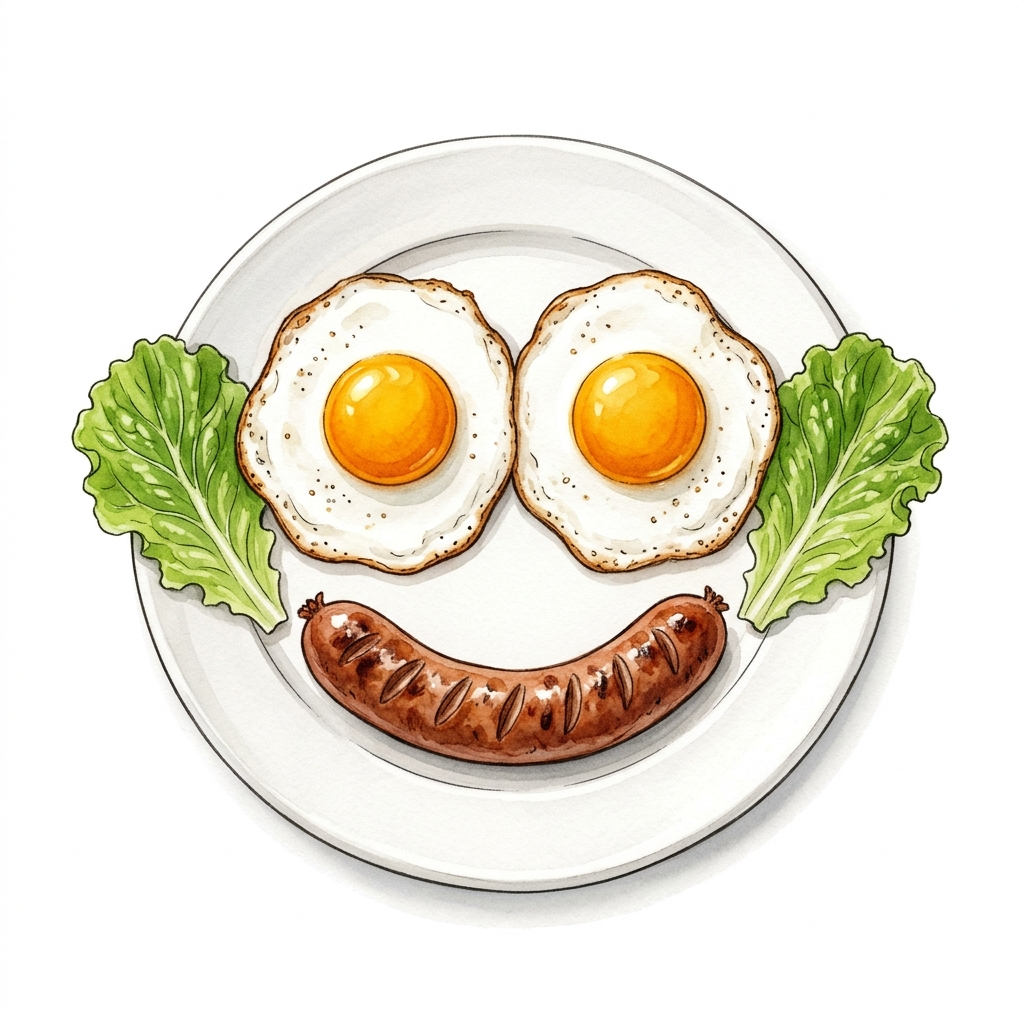
\includegraphics[width=0.85\linewidth]{vokab_300dpi/spigelee.png} \\
            \vspace{0.3cm}
    }}
    \vspace{0.4em}
    \textbf{\Large D'Spigelee (Pl. d'Spigeleeër)}\\
    \small\textit{(L'œuf au plat / The fried egg)}
\end{minipage}
\hfill
\begin{minipage}[t]{0.48\textwidth}
    \centering
    \textbf{\Large En Hunneg}
    \vspace{0.4em}
    \framebox{\parbox{0.88\linewidth}{\centering
            \vspace{0.3cm}
            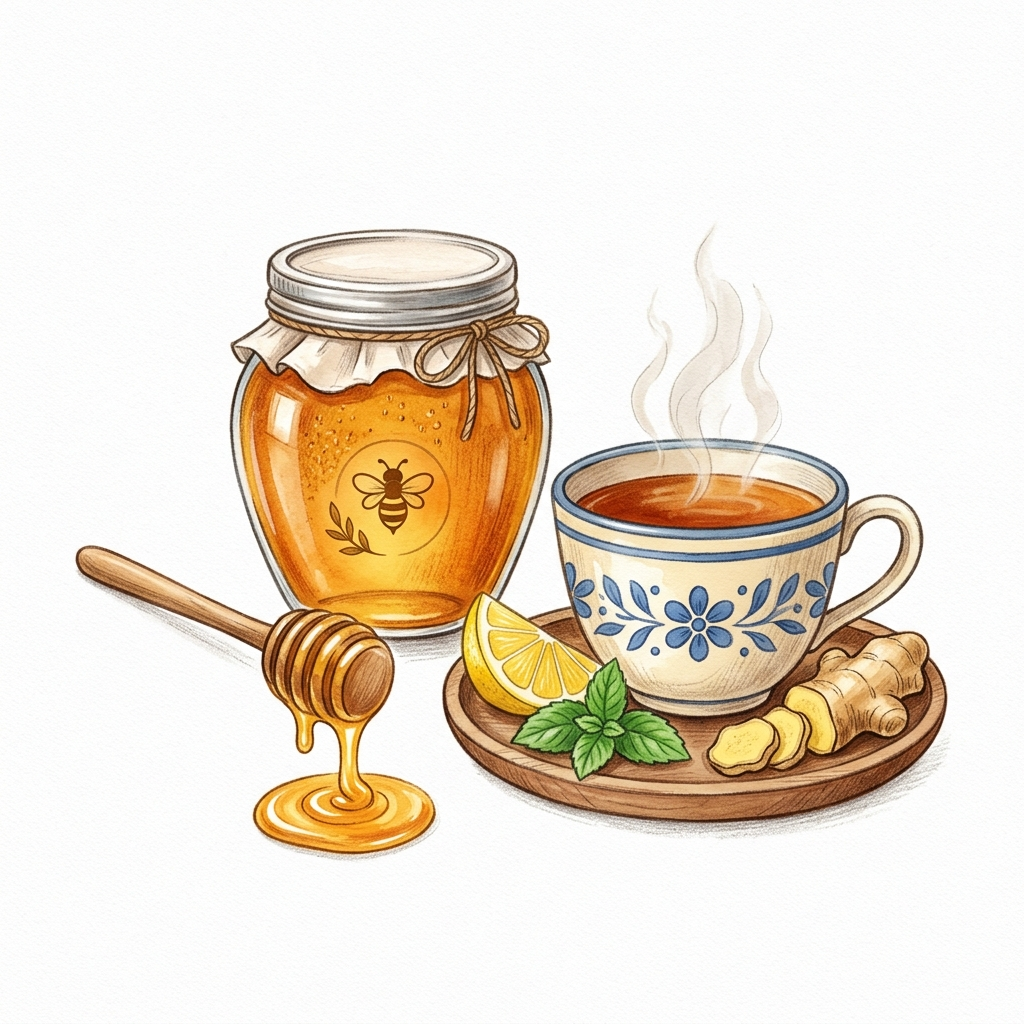
\includegraphics[width=0.85\linewidth]{vokab_300dpi/hunneg.png} \\
            \vspace{0.3cm}
    }}
    \vspace{0.4em}
    \textbf{\Large Den Hunneg (mam Téi a Peffermënz)}\\
    \small\textit{(Le miel / The honey)}
\end{minipage}
\end{noindent}

\vspace{2em}

\begin{noindent}
\begin{minipage}[t]{0.48\textwidth}
    \centering
    \textbf{\Large Eng Kanéngchen}
    \vspace{0.4em}
    \framebox{\parbox{0.88\linewidth}{\centering
            \vspace{0.3cm}
            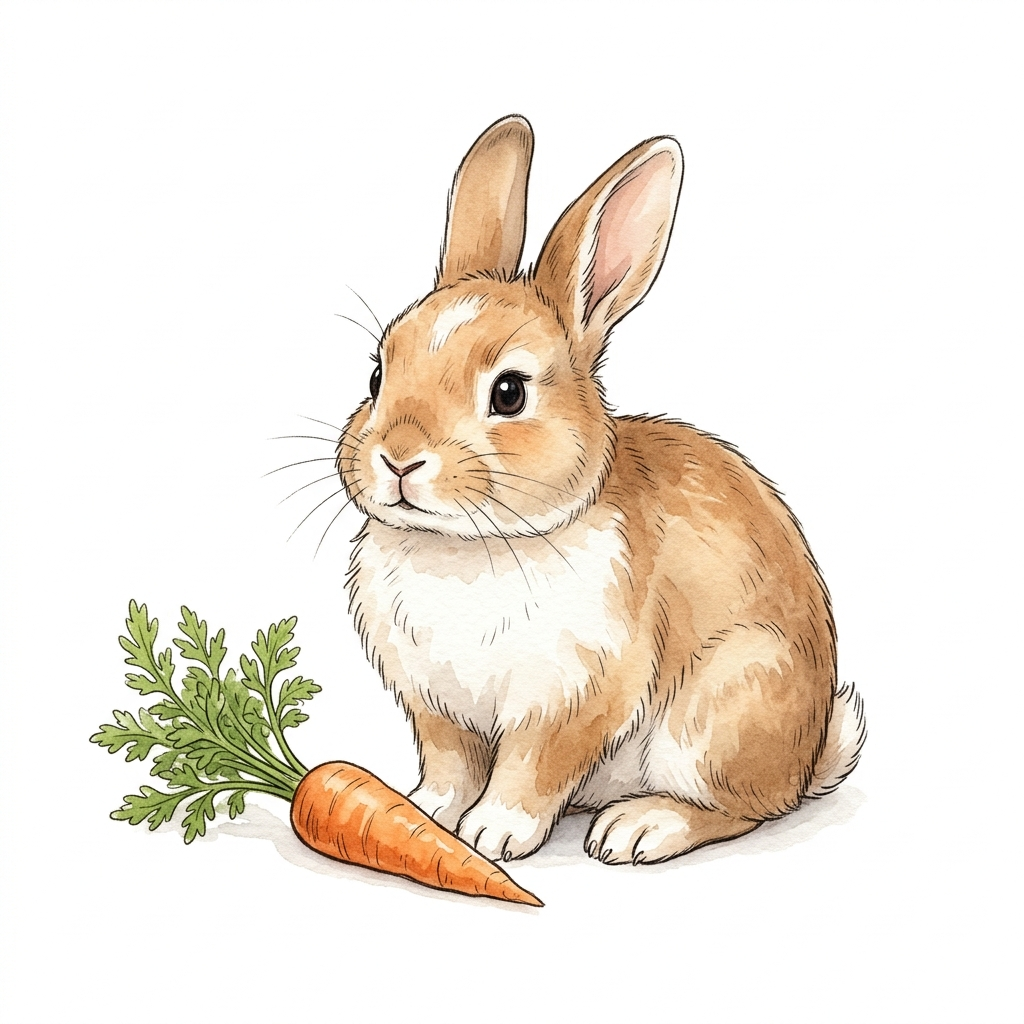
\includegraphics[width=0.85\linewidth]{vokab_300dpi/kanengchen.png} \\
            \vspace{0.3cm}
    }}
    \vspace{0.4em}
    \textbf{\Large D'Kanéngchen (Pl. d'Kanéngercher)}\\
    \small\textit{(Le lapin / The rabbit)}
\end{minipage}
\hfill
\begin{minipage}[t]{0.48\textwidth}
    \centering
    \textbf{\Large E Buch}
    \vspace{0.4em}
    \framebox{\parbox{0.88\linewidth}{\centering
            \vspace{0.3cm}
            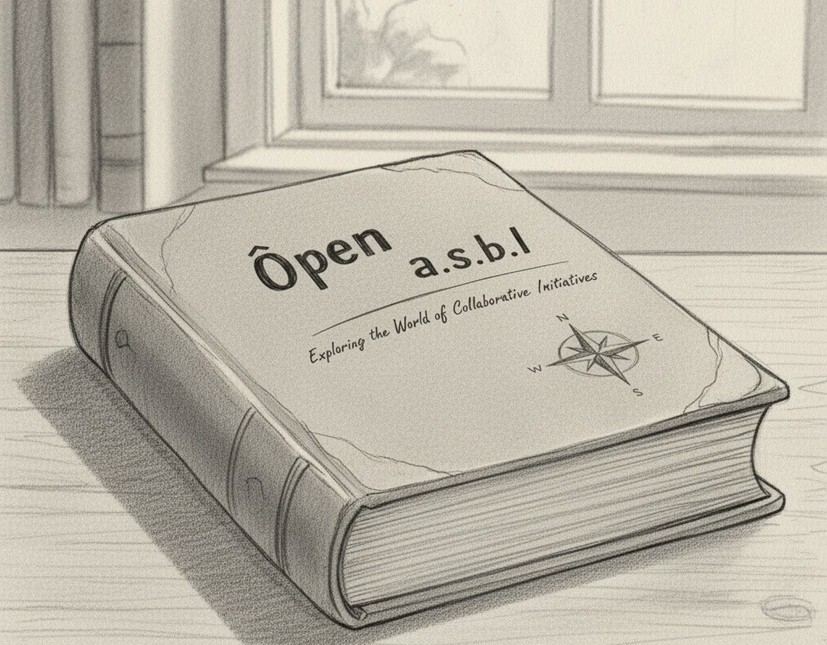
\includegraphics[width=0.85\linewidth]{vokab_300dpi/buch.png} \\
            \vspace{0.3cm}
    }}
    \vspace{0.4em}
    \textbf{\Large D'Buch (Pl. d'Bicher)}\\
    \small\textit{(Le livre / The book)}
\end{minipage}
\end{noindent}

\vspace{2em}

\begin{noindent}
\begin{minipage}[t]{0.48\textwidth}
    \centering
    \textbf{\Large E Poulet}
    \vspace{0.4em}
    \framebox{\parbox{0.88\linewidth}{\centering
            \vspace{0.3cm}
            
\includegraphics[width=0.85\linewidth]{vokab_300dpi/poulet.png} \\
            \vspace{0.3cm}
    }}
    \vspace{0.4em}
    \textbf{\Large De Poulet (Pl. d'Pouleten)}\\
    \small\textit{(Le poulet / The chicken)}
\end{minipage}
\hfill
\begin{minipage}[t]{0.48\textwidth}
    \centering
    \textbf{\Large Eng Fläsch}
    \vspace{0.4em}
    \framebox{\parbox{0.88\linewidth}{\centering
            \vspace{0.3cm}
            
\includegraphics[width=0.85\linewidth]{vokab_300dpi/Fläsch.png} \\
            \vspace{0.3cm}
    }}
    \vspace{0.4em}
    \textbf{\Large D'Fläsch (Pl. d'Fläschen)}\\
    \small\textit{(La bouteille / The bottle)}
\end{minipage}
\end{noindent}

\vspace{2em}

\begin{noindent}
\begin{minipage}[t]{0.48\textwidth}
    \centering
    \textbf{\Large E Bic}
    \vspace{0.4em}
    \framebox{\parbox{0.88\linewidth}{\centering
            \vspace{0.3cm}
            
\includegraphics[width=0.85\linewidth]{vokab_300dpi/bic.png} \\
            \vspace{0.3cm}
    }}
    \vspace{0.4em}
    \textbf{\Large De Bic (Pl. d'Bicen)}\\
    \small\textit{(Le stylo à bille / The ballpoint pen)}
\end{minipage}
\hfill
\begin{minipage}[t]{0.48\textwidth}
    \centering
    \textbf{\Large E Bläistëft}
    \vspace{0.4em}
    \framebox{\parbox{0.88\linewidth}{\centering
            \vspace{0.3cm}
            
\includegraphics[width=0.85\linewidth]{vokab_300dpi/blaisteft.png} \\
            \vspace{0.3cm}
    }}
    \vspace{0.4em}
    \textbf{\Large De Bläistëft (Pl. d'Bläistëfter)}\\
    \small\textit{(Le crayon / The pencil)}
\end{minipage}
\end{noindent}
